\documentclass[12pt, authoryear]{elsarticle}
\makeatletter
\def\ps@pprintTitle{%
	\let\@oddhead\@empty
	\let\@evenhead\@empty
	\def\@oddfoot{}%
	\let\@evenfoot\@oddfoot}
\makeatother
%\usepackage{lmodern}
% My spacing
\usepackage{setspace}
\setstretch{1.5}
\usepackage{multirow}
%\DeclareMathSizes{12}{14}{10}{10}
\usepackage[margin=2.5cm]{geometry}    % How to set margins - optimized for 2.5cm      

% See geometry.pdf to learn the layout options. There are lots.
\geometry{a4paper}                   			% ... or a4paper or a5paper or ... 
\usepackage{enumitem}
\usepackage{mathtools}
%\geometry{landscape}                		% Activate for rotated page geometry
\usepackage[parfill]{parskip}    			% Activate to begin paragraphs with an empty line rather than an indent
\usepackage{graphicx}						% Use pdf, png, jpg, or eps§ with pdflatex; use eps in DVI mode
% TeX will automatically convert eps --> pdf in pdflatex	
\usepackage{flafter}			
\usepackage{setspace}
%\linespread{1.5}
\usepackage[font={}]{caption}
\usepackage[bottom]{footmisc}
\usepackage[capposition=top]{floatrow}   %figure notes
\usepackage{lscape}
%math packages 
\usepackage{amssymb}
\usepackage{fancyhdr}
\usepackage{graphicx,epsf,subfigure}
\usepackage{pstricks,pst-node,psfrag}
\usepackage{amsthm,amssymb,amsmath}
\usepackage{amsmath,bm}

%mathnotes
\newcommand{\bbeta}{\mbox{\boldmath $\beta$}}
\newcommand{\beps}{\mbox{\boldmath $\epsilon$}}
\newcommand{\bX}{\mbox{\boldmath $X$}}
\newcommand{\bY}{\mbox{\boldmath $Y$}}
\newcommand{\bI}{\mbox{\boldmath $I$}}
\newcommand{\N}{\mathcal{N}}
\newcommand{\x}{\textsc{\textbf{x}}}
\newcommand{\xx}{\textsc{x}}
\definecolor{aurometalsaurus}{rgb}{0.43, 0.5, 0.5}
%add figure 
\DeclareGraphicsRule{.tif}{png}{.png}{`convert #1 `dirname #1`/`basename #1 .tif`.png}
\usepackage{rotating}
\usepackage{pdflscape}
\usepackage{hyperref}
\usepackage[round]{natbib}
	\definecolor{ashgrey}{rgb}{0.7, 0.75, 0.71}
\usepackage{soul}

\def\bibsection{\section{References}} %%% Make "References" appear before bibliography
\usepackage{longtable}
\usepackage{hyperref}
\usepackage{tablefootnote}
\usepackage{lscape} 
\usepackage{animate}

\renewcommand{\contentsname}{Table of Contents} % change name from Contents to Table of Contents

\usepackage{titlesec}

\setcounter{secnumdepth}{4}

%_______________________________________________________________________________________________________%
%_______________________________________________________________________________________________________%
%\usepackage[table]{xcolor}% http://ctan.org/pkg/xcolor
%\usepackage{graphicx,multirow}
\usepackage{xcolor,colortbl}
\usepackage{xcolor}
%\usepackage{graphicx,multirow}
\usepackage[capposition=top]{floatrow}
\setcounter{secnumdepth}{4}
\usepackage{tikz}
\begin{document}

\begin{frontmatter}  %

\title{When it Hurts: \\ \vspace{0.5cm} \large Demand Estimation in the U.S Analgesics Market}

\author[Add1]{Reid Falconer}
\ead{reid.falconer@bracelonagse.eu}

\author[Add1]{Eric Beckwith}
\ead{eric.beckwith@bracelonagse.eu}

\author[Add1]{Felix Adam}
\ead{felix.adam@bracelonagse.eu}
\author[Add1]{Maryam Rahbaralam}
\ead{maryam.rahbaralam@bracelonagse.eu}

\address[Add1]{Barcelona Graduate School of Economics, Barcelona, Spain}
%\address[Add2]{Some other Institution, Cape Town, South Africa}

%\cortext[cor]{Corresponding author: Nico Katzke}

%\begin{abstract}
%\small{
%Abstract to be written here. 
%}
%\end{abstract}

%\vspace{1cm}

\begin{keyword}
\footnotesize{
Demand Estimation  \sep OTC Analgesics \sep  Nested Logit Model \\ \vspace{0.3cm}
%\textit{JEL classification} L250 \sep L100
}
\end{keyword}
\vspace{0.5cm}
\end{frontmatter}

\headsep 35pt % So that header does not go over title


\section{Introduction} \label{introduction}
Demand analysis of the market for over the counter (OTC) analgesics, better known as painkillers, offers valuable insights into what drives the demand for painkillers, how consumers tend to be influenced by prices and product differentiation. Furthermore, these insights have potential use for marketing and management strategies.

The market for painkillers can be considered vastly different from other consumer goods available in supermarkets such as soda or cereals. It is not entirely clear, whether OTC painkillers should be regarded as normal or necessary goods. It could be, that the demand for painkillers rises with falling prices, due to greater affordability. On the other hand, one could argue that, given proper use, painkillers are almost independent of prices, since consumers only use them when needed. Moreover, the market for painkillers is clearly segmented by natural groupings, given by the active substance in the drug.

In this work we present an analysis of demand patterns for analgesics in the U.S market, using scanner data. We build on the extensive Dominick’s Dataset which provides weekly scanner data from 56 stores of Dominick’s Finer Foods in the Chicago area from 1990 to 1997. Besides weekly sales and price data, the data set includes extensive information on customer demographics as well as many economic indicators.

The focus of our work lies on estimating price elasticities for painkillers as well as identifying other drivers of painkiller sales. As aforementioned, painkillers can be naturally grouped by their active ingredient and consequently, we estimate own- and cross-price elasticities using a nested logit model that is close in spirit to that of \cite{berry1994estimating}.

Our results show that the grouping by active ingredients carries over to the observed demand patterns. Cross-price elasticities obtained from the nested logit model display low rates of substitution across different substances, while elasticities inside the groups are significantly larger. Since observed market shares remain stable over time, we assume that consumers have strong preferences towards active substances, but not for certain products within a group. 

The outline of this paper is as follows: firstly, an overview of the U.S analgesics market is provided along with a description and statistical analysis of the data. Section \ref{method}  provides an in-depth discussion of the methodological approach and Section \ref{results} presents the results. Finally, Section \ref{conclusion} concludes.


\section{The U.S OTC Analgesics Industry and Data}\label{data}

Over-the-counter (OTC) analgesics or painkillers are non-prescription drugs to treat fever and pain. Painkillers come in three main active ingredients:  acetaminophen (called paracetamol in the U.K.) aspirin and ibuprofen. The active ingredients may vary in the kinds of pains they relieve and in their side effects. Acetaminophen treats most pains and fevers and is known for having little side effects. Ibuprofen also treats most pains and fevers and is often used to reduce inflammations, but it may have side effects on the stomach. Aspirin also has a blood-diluting effect, which has both advantages and disadvantages. While each active substance may, therefore, relieve pain and reduce fever in different ways and with varying side effects, consumer perceptions of the brands (branded vs generic) may also be important. This is evident from a large amount of advertising in the sector. So it is ultimately an empirical question to which extent brands within different active ingredients are substitutes.

The OTC analgesics industry is concentrated such that five firms account for approximately 95\% of the market share in dollar terms \footnote{Excedrin is omitted in this analysis, given that their main product includes both aspirin and
acetaminophen as active ingredients.}. Tylenol is the industry leader with a market share of approximately 42\% while generic firm, Dominick's, only accounts for 23.9\% of the market. Table \ref{active_share} gives a  breakdown of the sample used in this study and shows the market shares of the three active ingredients. With a market share of 52\%, acetaminophen is by far the most important ingredient. Ibuprofen and aspirin each have a market share of approximately 34\% and 14\% respectively.

\begin{table}[H]
	\caption{Market Shares by Active Ingredients}
	\label{active_share}
	\begin{tabular}{cc} \hline  \hline
		\textbf{Active Ingredient}  \cellcolor{gray!25} & \textbf{Market Share}  \cellcolor{gray!25} \\ \hline
		Aspirin & 14.30\% \\
		Ibuprofen & 33.80\% \\
		Acetaminophen & 51.90\% \\ \hline \hline
		\multicolumn{2}{c}{Source: Dominick's dataset}     
	\end{tabular}
\end{table}

Interestingly, each firm predominately specialises in one active ingredient. Table \ref{mshare}  presents the market shares of the firms, together with their products and active substance. This illustrates that Tylenol and Dominick's are the only two firms within the acetaminophen segment: Tylenol sells X/S Caplets as its main product, whereas Dominick's sells ibrupofen as its primary product. Moreover, Advil is the main firm within the ibrupofen segment while Anacin and Bayer are the only two firms that are solely based in the aspirin market. 

% Please add the following required packages to your document preamble:
% \usepackage{multirow}
% \usepackage{graphicx}
\begin{table}[H]
	\caption{Market Shares by Firms, Products and Active Ingredients}
	\label{mshare}
	\resizebox{\textwidth}{!} & Dom Coated Aspirin & Aspirin & 5.20\% \\
			&  & Dom E/S Non-Asp Caplet & Acetaminophen & 4.80\% \\
			&  & Dom Ibuprofen & Ibuprofen & 9.30\% \\
			&  & Dom X/S Non-Asp & Acetaminophen & 4.60\% \\ \hline
			\multirow{4}{*}{\textbf{Tylenol}} & \multirow{4}{*}{42.50\%} & Tylenol X/S Caplet & Acetaminophen & 15.00\% \\
			&  & Tylenol X/S Gelcaps& Acetaminophen & 13.80\% \\
			&  & Tylenol X/S Tablets & Acetaminophen & 9.40\% \\
			&  & Tylenol X/S Tabs & Acetaminophen & 4.30\% \\ \hline
			\multirow{2}{*}{\textbf{Advil}} & \multirow{2}{*}{24.40\%} & Advil & Ibuprofen & 14.80\% \\
			&  & Advil Caplet & Ibuprofen & 9.60\% \\ \hline
			\textbf{Anacin} & 4.50\% & Anacin Tabs & Aspirin & 4.50\% \\ \hline
			\textbf{Bayer} & 4.60\% & Bayer Aspirin & Aspirin & 4.60\% \\ \hline \hline
					\multicolumn{5}{c}{Source: Dominick's dataset}   
		\end{tabular}%
	}
\end{table}

\subsection{Data}

The primary data used in this study is drawn from the Dominick's dataset. The dataset covers store-level scanner data collected at Dominick's Finer Foods over a period of seven years. Specifically, the dataset consists of weekly observations of the prices, sales and market shares of OTC analgesics in the Chicago metropolitan area for 343 weeks, from January 1992 to December 1998. The observations are defined as product-week-store combinations, and the data contains essential product attributes: active ingredient, pill type (caplet, tablet, gelcap, etc.) and the number of pills contained in the product. Additionally, the data is supplemented with demographic data at the store level.

The quantity sold was computed by summing weekly total units sold within each store and dividing that by the size of the package (i.e. size adjusted units sold, given that some firms have different package sizes). Additionally, since the actual prices were missing, unit values were used as a proxy for them. To compute unit values, prices were calculated at the store level for each product, as total revenue for the product in the store in a week divided by the total number of products sold in that week \footnote{Note that expenditures are further adjusted by subtracting the value of coupons (if any)}. Furthermore, all prices (unit values) were adjusted for inflation by dividing them by the weekly regional Consumer Price Index (CPI).

Over the study period, the average total weekly amounts of analgesic sold by Dominick's, Tylenol, Advil, Anacin and Bayer, were 408, 251, 215, 331  and 369 units, respectively, indicating that Dominick’s was the leading firm followed by Bayer, Anacin, Tylenol and Advil. Furthermore, this firm ordering is identical when evaluating the firm's median weekly prices per unit with Dominick's and Bayer having the two lowest median weekly prices per unit within the market respectively (See: Figure \ref{p_v_s}).

\begin{figure}[H]
	\centering
	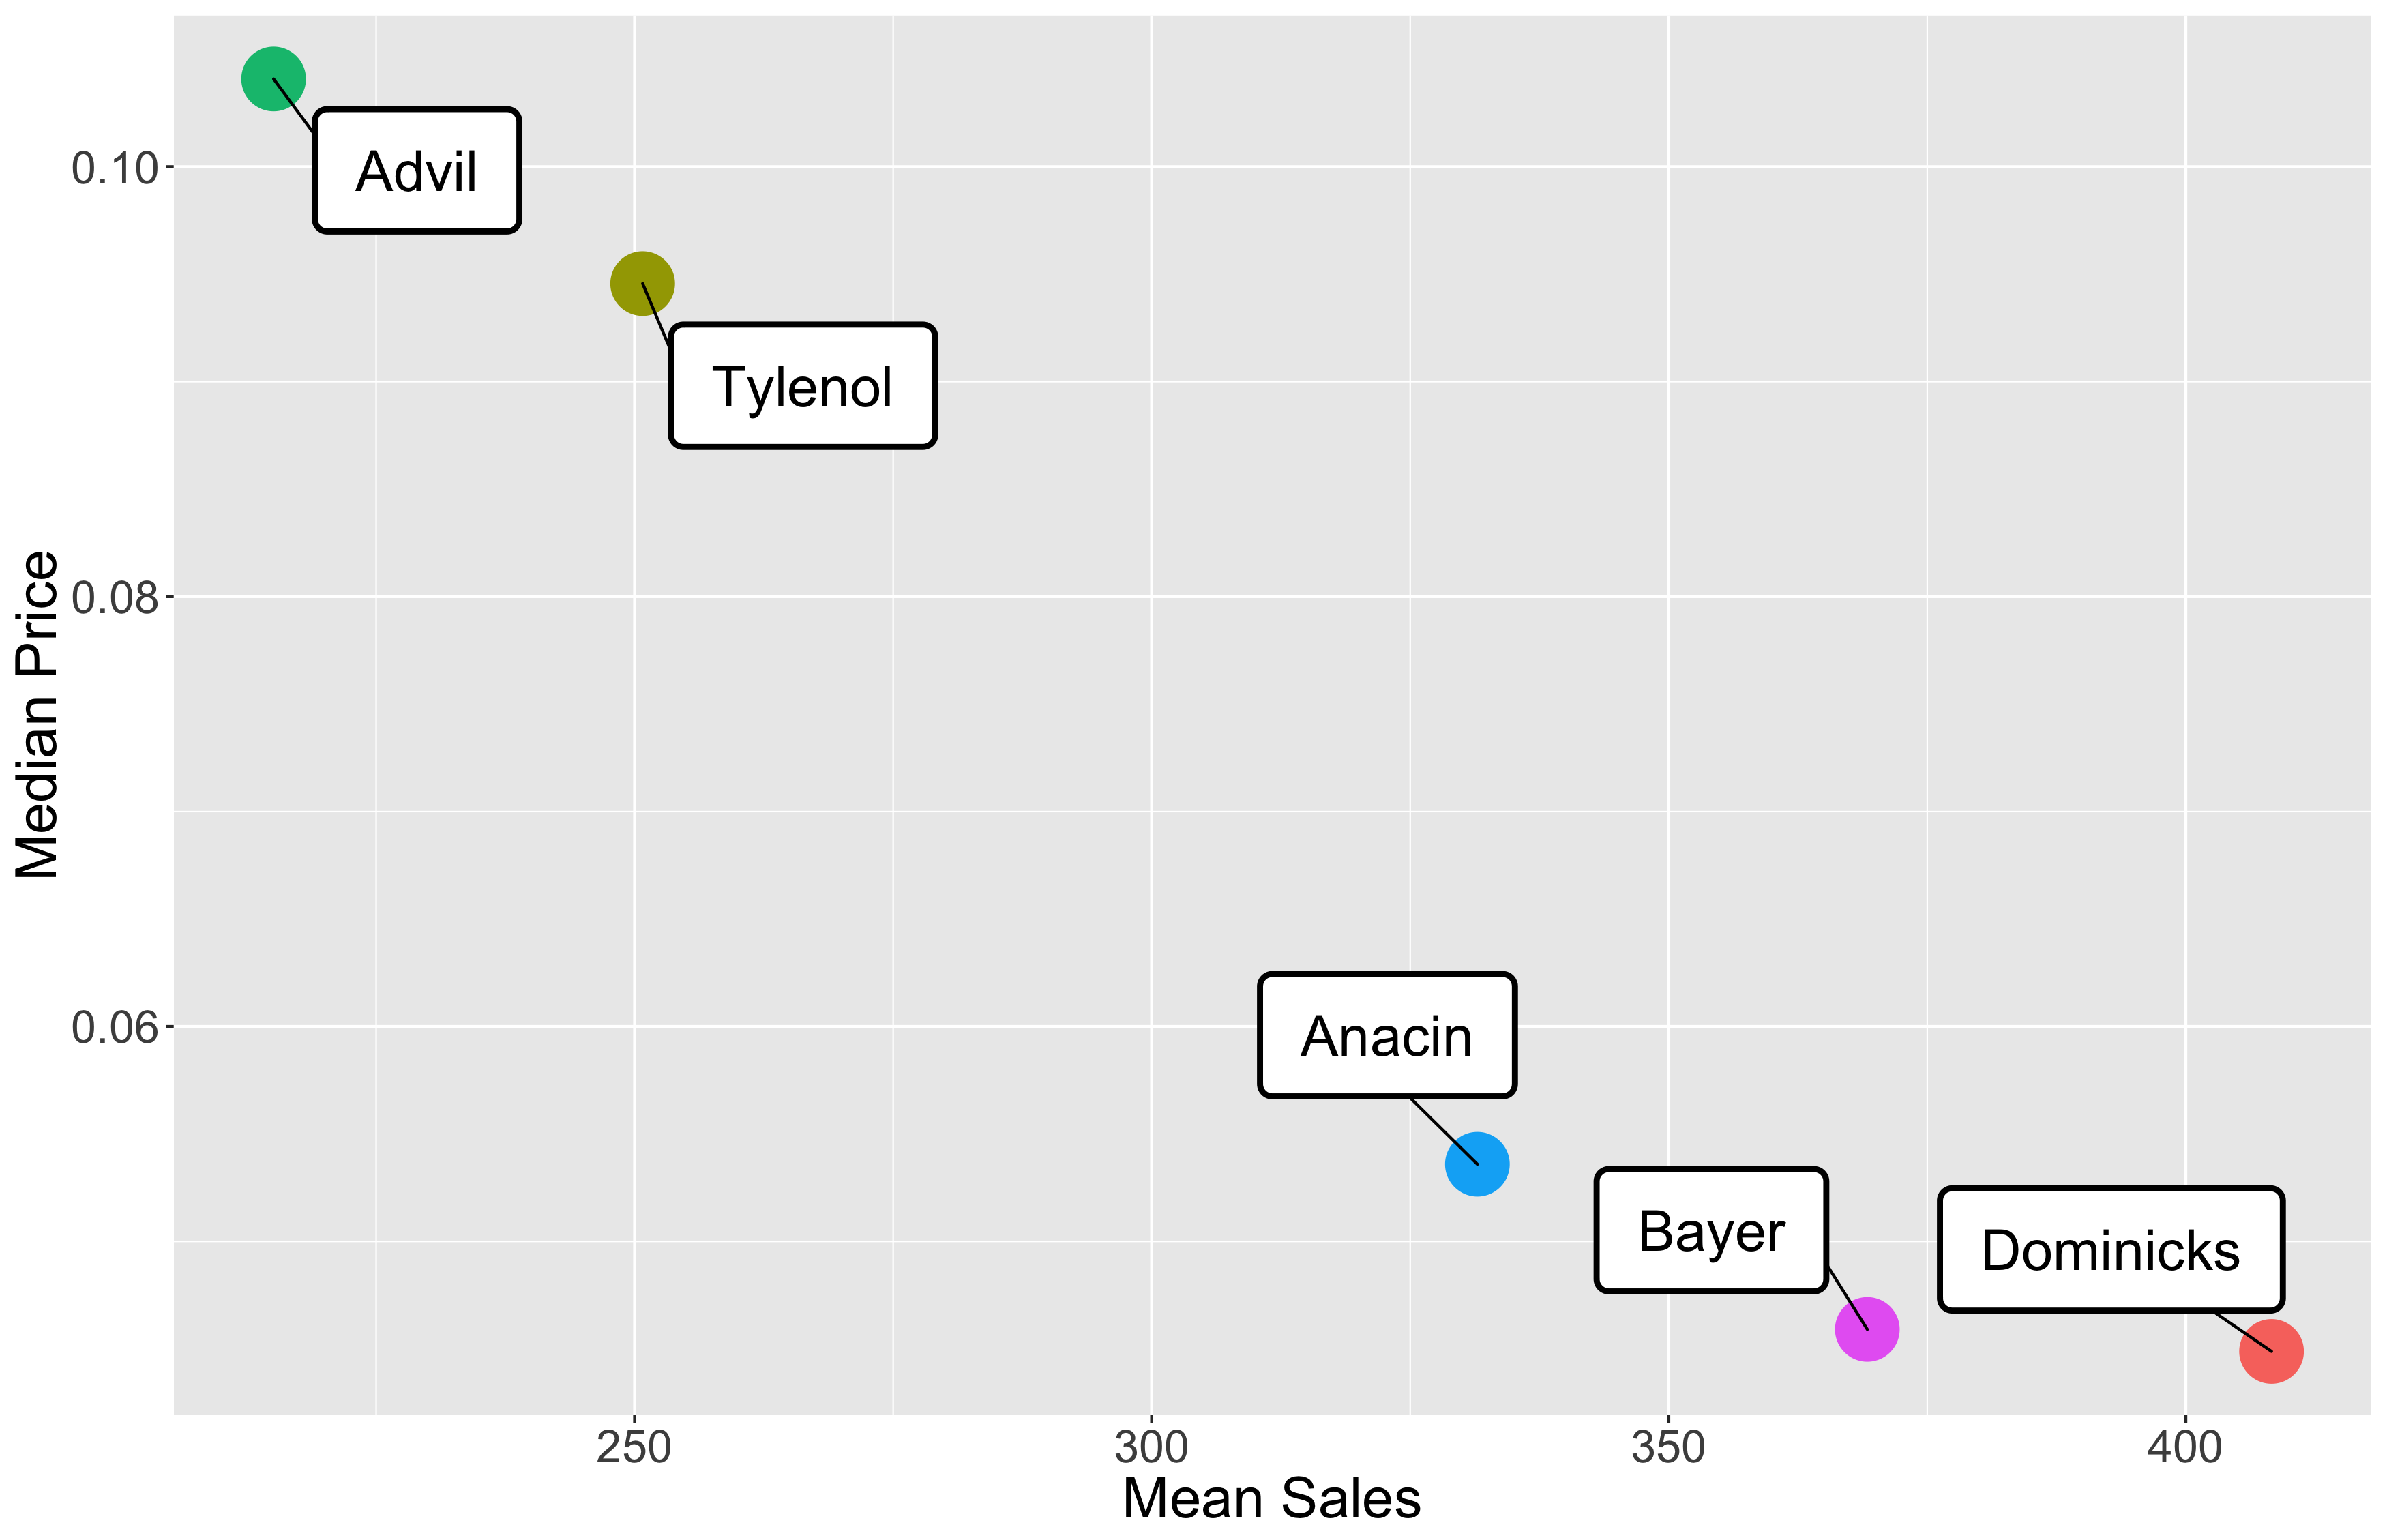
\includegraphics[clip, angle=0, width=12cm]{firm_plot.png}
	\caption{ Median Price vs Average Sales by Firm}\label{p_v_s}
\end{figure}

Figure \ref{new} shows that the grouping by the active substance can also be found in the price and sales data. The three groups clearly stand out, with ibuprofen having the highest median prices, followed by acetaminophen and aspirin. Moreover, all plots show signs of downward sloping demand curves.

\begin{figure}[H]
	\centering
	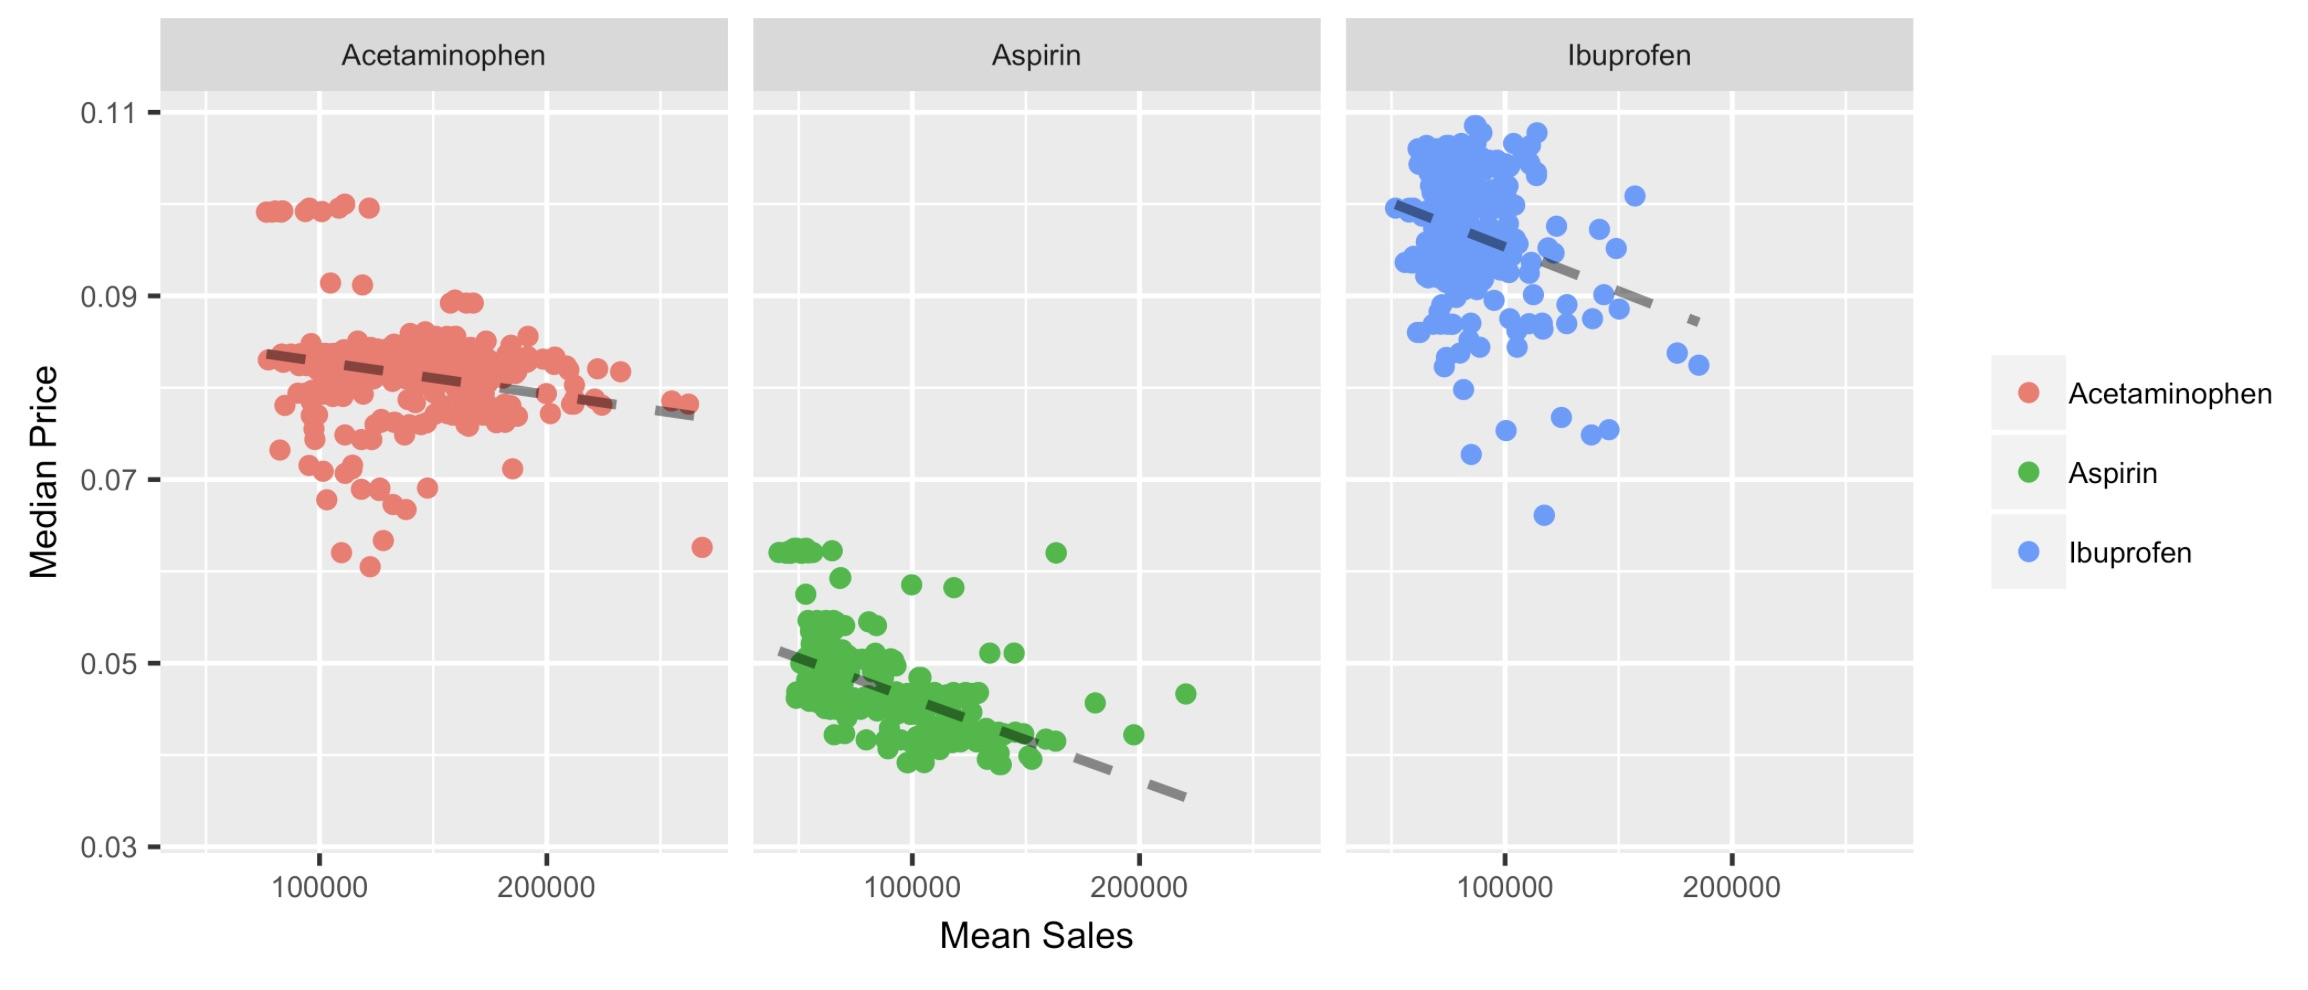
\includegraphics[clip, angle=0, width=1\textwidth]{active_sub_scatter.jpg}
	\caption{ Median Price vs Average Sales by Active Ingredient }\label{new}
\end{figure}

The market shares by percentage of total quantity sold can be seen in Figure \ref{new2}. Here we see, that the market shares by active ingredient don't vary substantially over time. Acetaminophen has the highest market share, followed by ibuprofen and aspirin. The shares almost remain constant over the whole time frame, with only little deviations.

\begin{figure}[H]
	\centering
	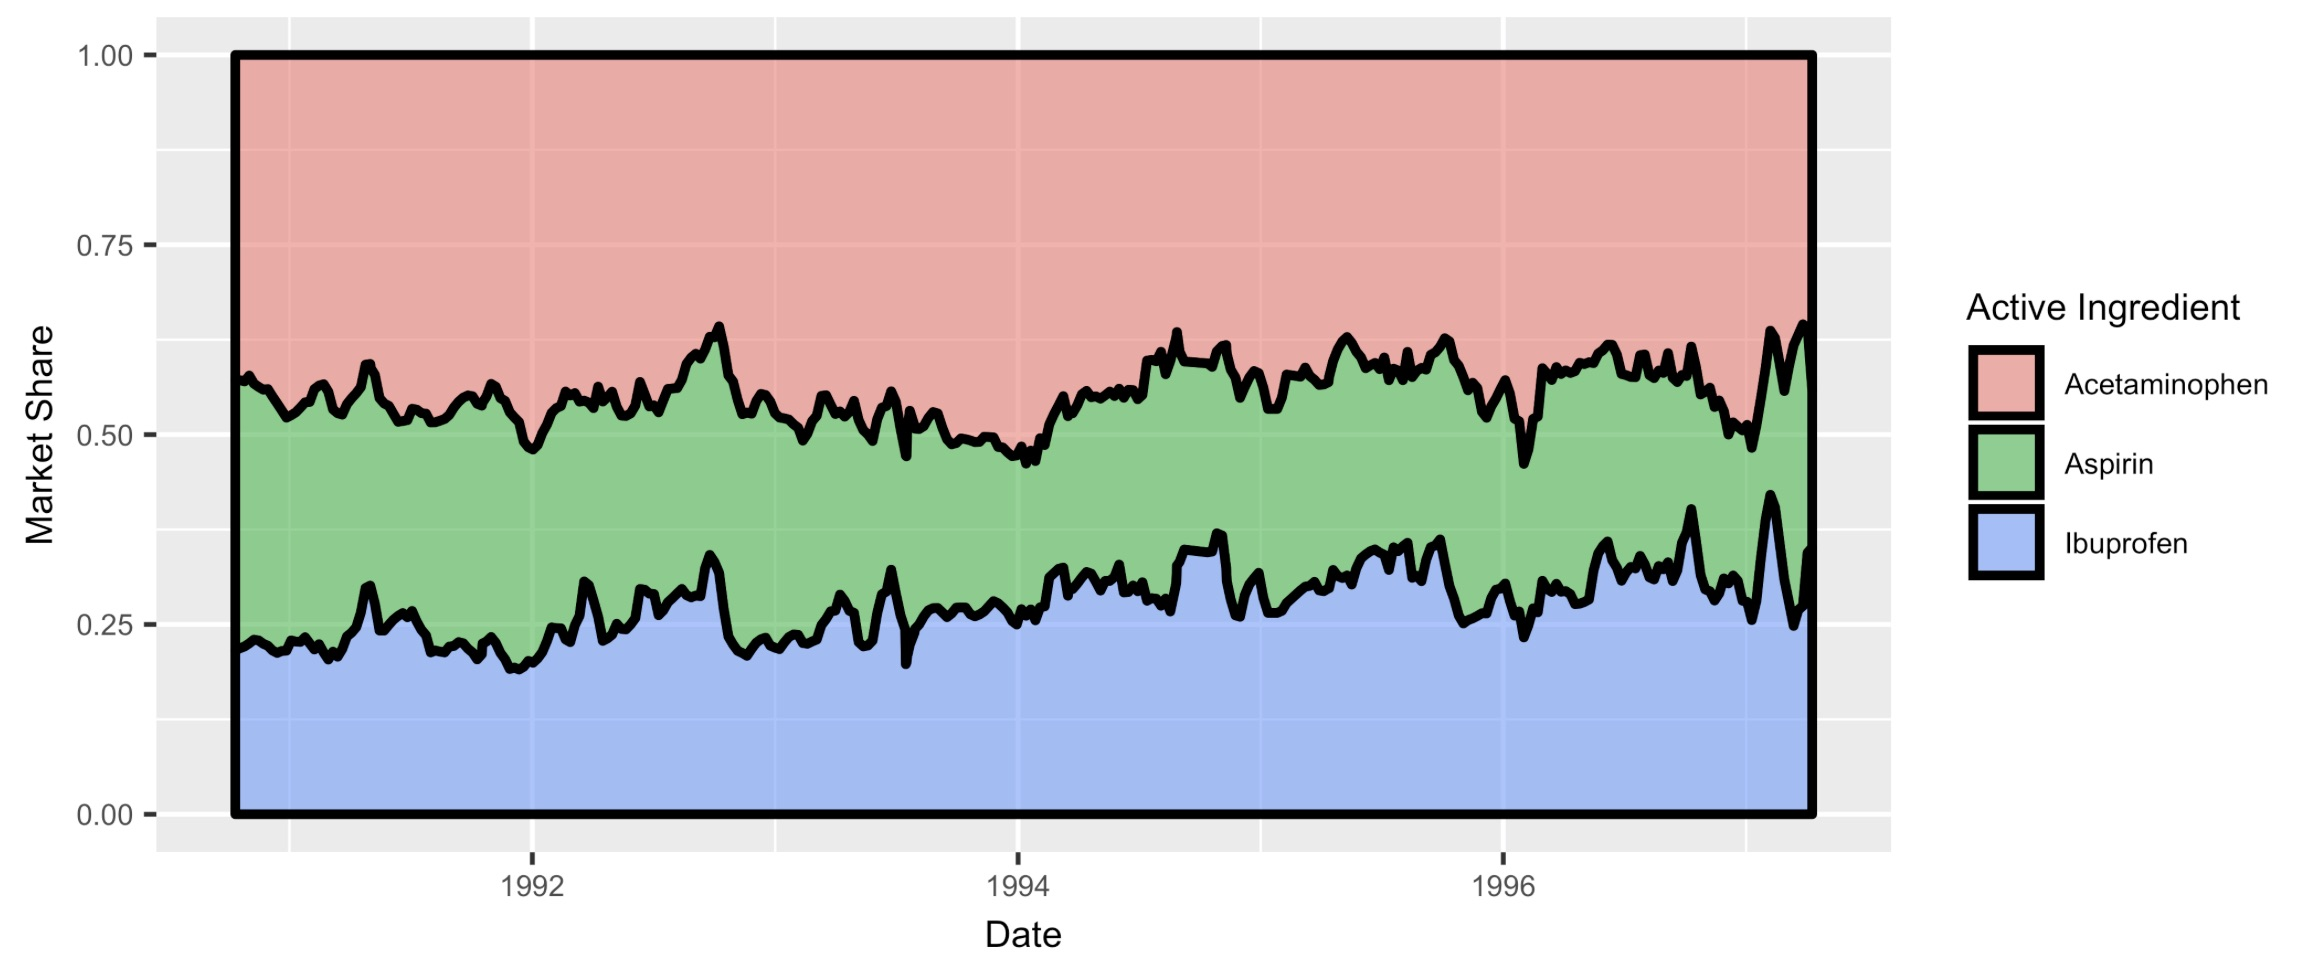
\includegraphics[clip, angle=0, width=1\textwidth]{market_share.jpg}
	\caption{ Market Shares by Active Substance (\%Of Qty Sold)}\label{new2}
\end{figure}

\section{Methodological Approach} \label{method}
\subsection{Econometric Set Up} 

The findings described in Section \ref{data} lead us to our econometric setup. We make use of a nested logit model as described by \cite{mcfadden1978modeling}, \cite{cardell1997variance} and \cite{berry1994estimating}. We begin by motivating the use of the nested logit model, then describe our econometric setting and finally discuss instrumental and control variables.

\cite{mcfadden1978modeling} analyses the behaviour of consumers with regard to choosing a residential location. While the choice of painkillers and housing seem very distant at first, we argue that the nested logit model used by McFadden offers some valuable insights into the painkiller market. \cite{mcfadden1978modeling}  argues, that consumers choose their residential location by maximising the utility they receive from a particular house. This utility depends on the characteristics, such as location, number of rooms and the community. Additionally, the consumer is faced with choosing exactly one house or none \citep{mcfadden1978modeling}.

The idea that consumers maximise utility with respect to product characteristics translates easily to the painkiller market. Consumers choose painkillers dependent on their tolerance for specific active ingredients (i.e. aspirin, acetaminophen and ibuprofen) and their brand preferences (i.e. branded vs generic). The second assumption, consumers only buy one good or none (the outside good), can also be motivated through properties specific to painkillers.

While it is possible to take combinations of certain painkillers, it is generally not recommended to do so, only if indicated by medical advice. The simultaneous intake of aspirin and ibuprofen is associated with an increased risk of stomach bleeding, or other side effects  \citep{miller1981combination}. Furthermore, we assume that consumers buy painkillers to tackle a specific problem, such as headaches or light fever.

Under rational behaviour, consumers will, therefore, buy the product which best suits their needs. This phenomenon is inherently different from other product categories, such as sodas, where one could imagine that consumers purchase different types of sodas at the same time. Moreover, including the choice of the outside good makes sense from the modelling and consumer perspective. It seems sensible to assume that in any given week, many consumers choose not to buy any painkillers at all, since they don’t experience any health issues. Including the outside good also simplifies the estimation of the structural demand parameters, as discussed in \cite{berry1994estimating}.

Another critical assumption made by \cite{mcfadden1978modeling} is that consumer tastes are correlated across products. In the case of housing, the similarities are shared across communities, where houses in the same community share specific characteristics \citep{mcfadden1978modeling}). Given that painkillers can be easily grouped by their active ingredient, this assumption translates well to our setting. We expect that consumer and product characteristics are correlated inside the groups. For example, some consumers might be more inclined to buy painkillers containing ibuprofen than aspirin, be it for medical or digestibility reasons.

Now that the conceptual framework has been set, we present the empirical model.

\subsection{The Empirical Model} 
As described, the nested logit model arises from the choice a consumer faces when buying painkillers. Each consumer bases their choice of painkiller on the utility they receive from it. We group products into four groups $g \in G = \{ A, P, I, O \}$ where A aspirin, P is paracetamol, and I is ibuprofen.  (See Figure \ref{tree1}). 

\begin{figure}[H]
	\centering
	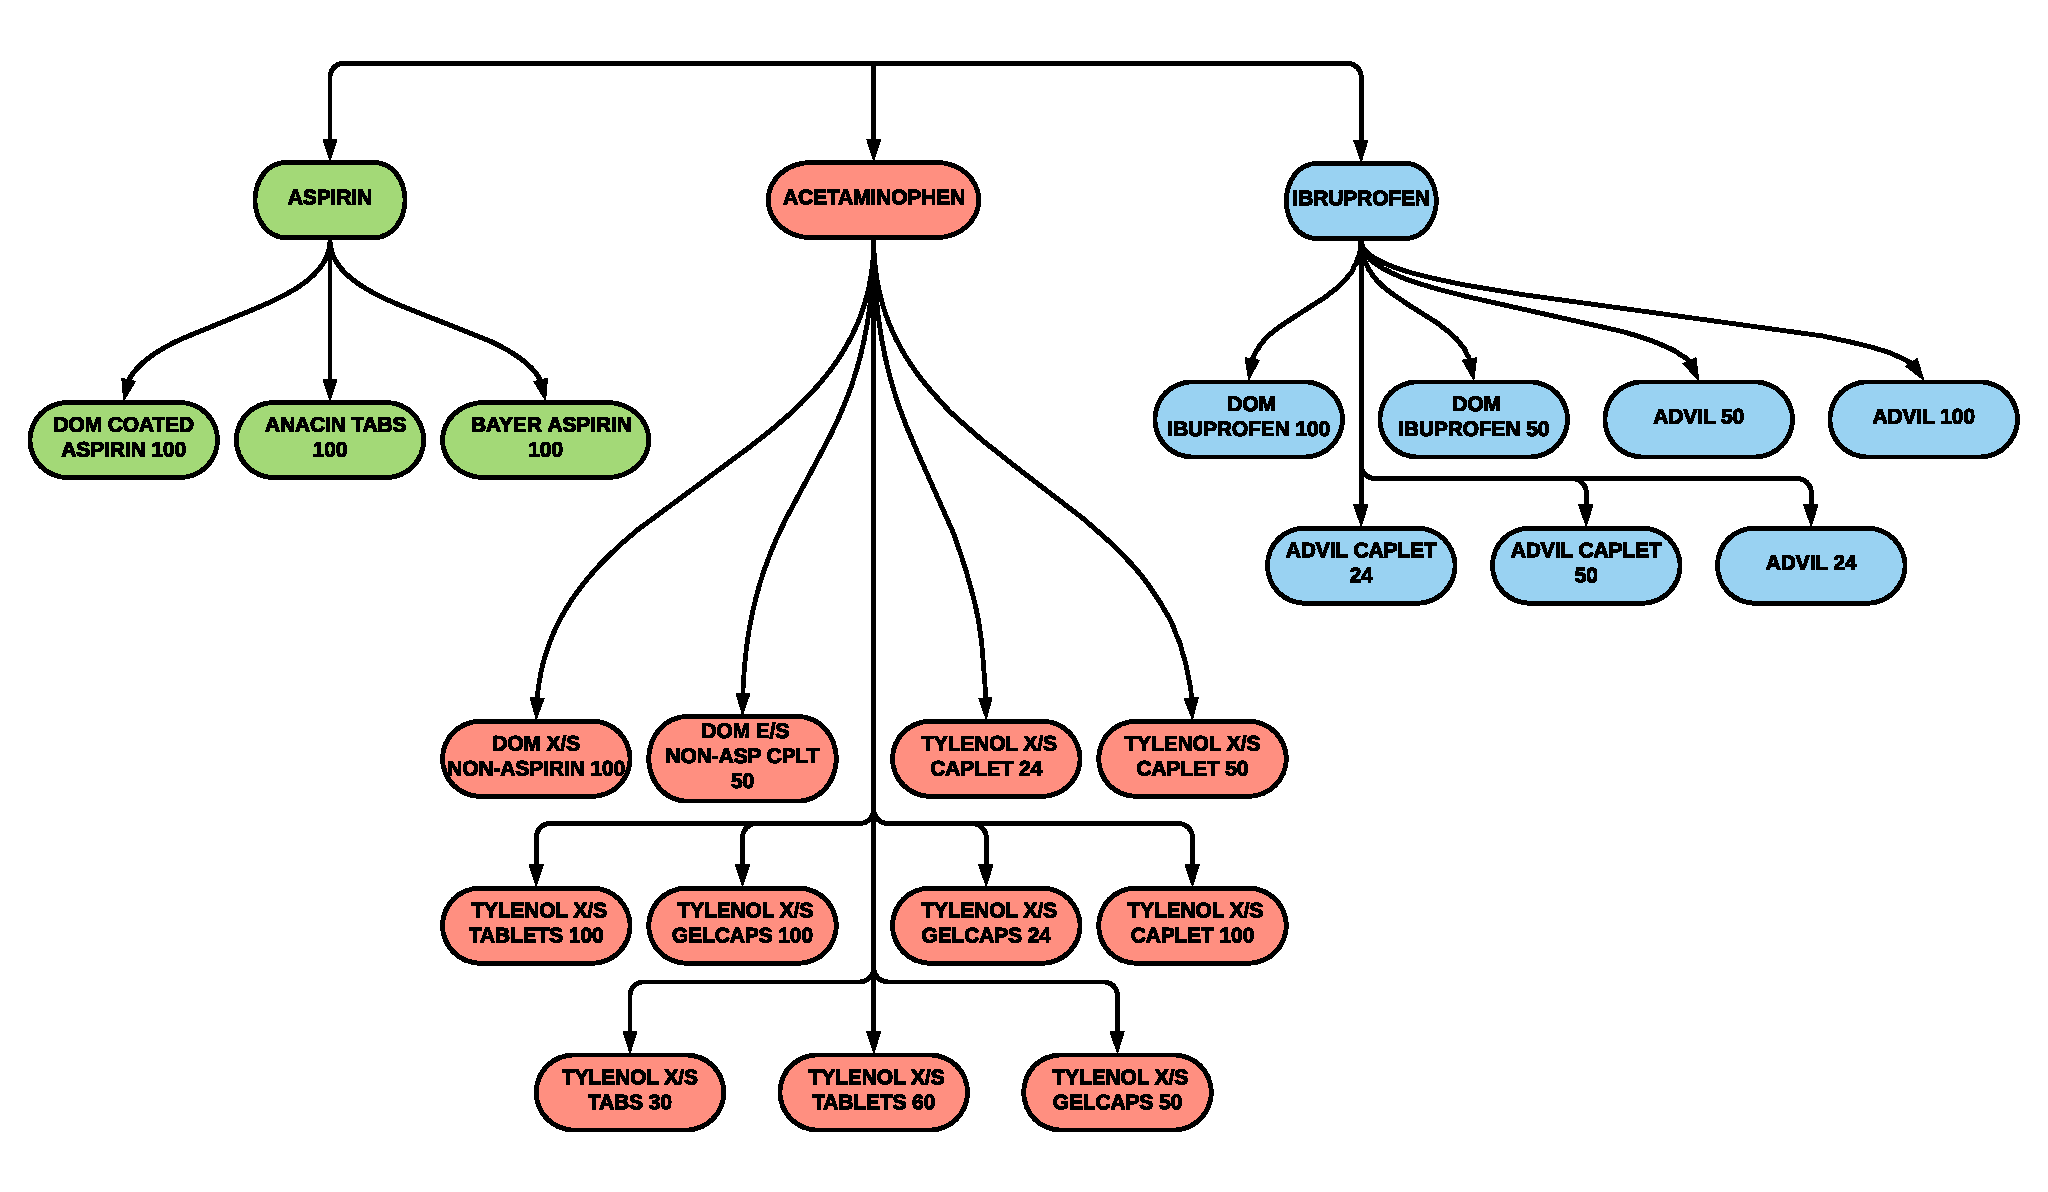
\includegraphics[clip, angle=0, width=1\textwidth]{FIG1.pdf}
	\caption{Tree structure of the active ingredient nested logit model}\label{tree1}
\end{figure}

Group $g = O$ denotes the choice the outside good. Consumers $i$'s utility $u_{ij}$ of consuming product $j$ is defined as: 

\begin{equation}
u_{ij} = X_j \beta - \alpha p_j + \xi _{j} + \xi _ {ig} + (1- \sigma)\epsilon_{ij}
\end{equation} 

Where $p_j$ denotes the price of product $j$, $\xi_{i}$ are product characteristics specific to product $j$, $\xi_{ig}$ are common properties for all products in group $g$ and $\epsilon_{ij}$ is the error term assumed to have an extreme value distribution.The Parameter $\sigma$, which
is $0 \leq \sigma < 1$, determines the ``within group'' correlation. If $\sigma$ approaches one, the correlation
among brands within a group becomes one, meaning that the consumer is only concerned with choosing a group, not products within the group. If $\sigma$ approaches zero, the ``within group'' correlation becomes zero, which is equivalent to the simple multinomial logit model (Berry, 1994). 

We assume that consumer $i$ purchases brand $j$ if $ { u } _ { { ij } } >  { u } _ {  { ik } } ,$ Where $\mathrm { \forall } \mathrm { k } \neq \mathrm { j }$. If $\varepsilon _ { \mathrm { ij } }$ follows a generalized
extreme value distribution, the market share of product $j \in g$ within group $g$ is derived as follows:
\begin{equation}
s _ { j | g } ( \vec { \delta } , \sigma ) = \frac { \exp \left( \delta _ { j } / ( 1 - \sigma ) \right) } { D _ { g } }
\end{equation}
where $D _ { g } \equiv \sum _ { j \in \mathcal { G } _ { g } } \exp \left( \delta _ { j } / ( 1 - \sigma ) \right)$.
Similarly, the probability of choosing group $g$ is:
\begin{equation}
s _ { g } ( \vec { \delta } , \sigma ) = \frac { D _ { g } ^ { ( 1 - \sigma ) } } { \left[ \sum _ { k } D _ { k } ^ { ( 1 - \sigma ) } \right] }
\end{equation}
Accordingly, the market share of product $ { j } \in \mathrm { g }$ can be derived from the following relationship:
\begin{equation}
\mathrm { s } _ { \mathrm { j } } = \mathrm { S } _ { \mathrm { j } / \mathrm { g } } \cdot \mathrm { S } _ { \mathrm { g } }
\end{equation}
Meanwhile, the market share of the "outside good" is:
\begin{equation}
s _ { 0 } ( \vec { \delta } , \sigma ) = 1 / \left[ \sum _ { k } D _ { k } ^ { ( 1 - \sigma ) } \right]
\end{equation}
In this nested logit framework, the independence of irrelevant alternatives (IIA) assumption holds. In the following, we show the calculations of the price elasticities.
Taking the logs of market shares we derive our empirical model:
\begin{equation}
\begin{aligned} \ln \left( s _ { j } \right) - \ln \left( s _ { 0 } \right) & = \delta _ { j } + \sigma \ln \left( s _ { j | g } \right) \\ & = \vec { x } _ { j } \vec { \beta } - \alpha p _ { j } + \sigma \ln \left( s _ {j | g } \right) + \xi _ { j } \end{aligned}
\end{equation}

We can then derive the own- and cross price elasticities from our estimated parameters:

$\frac { \partial s _ { j } } { \partial p _ { k } } \frac { p _ { k } } { s _ { j } } = \left\{ \begin{array} { l l } { - \alpha p _ { j } \left( 1 - \sigma s _ { j | g } - ( 1 - \sigma ) s _ { j } \right) / ( 1 - \sigma ) , } & { \text { if } k = j } \\ { - \alpha p _ { k } \left( \sigma s _ { j | g } + ( 1 - \sigma ) s _ { k } \right) / ( 1 - \sigma ) , } & { \text { if } j , k \in g } \\ { \alpha p _ { k } s _ { k } , } & { \text { otherwise } } \end{array} \right.$

However, the presence of unobserved characteristics creates the well-known problem of price endogeneity: if consumers and firms know the values of unobserved product characteristics  $\xi _ { j \mathrm { t } }$, while we (the econometricians) do not, then prices ($p_j$) are likely to be correlated with these unobservables. Additionally, in the nested logit model, the  nesting term ln$\left( s _ { j / g  } \right)$ is endogenous by construction, since any shocks to $\xi _ { j \mathrm { t } }$ that increase the dependent variable $\ln \left( s _ { j } \right) - \ln \left( s _ { 0 } \right)$  will also increase the nesting term ln$\left( s _ { j / g  } \right)$.

\subsection{Endogeneity Bias and Instrumental Variables}

Our primary interest lies in estimating the causal effect of price changes on market shares, as this effect will allow us to obtain meaningful elasticities estimates. 

In addition to the above-mentioned sources of endogeneity within our model, prices and quantities are determined by the intersection of demand and supply curves. However, it is not clear, whether demand or supply shocks drive the changes observed in quantities and prices. It could be, that a sudden positive demand shock, due to a flu pandemic, shifts the demand curve outward and therefore drives up prices. Similarly, sudden supply shocks could also lead to price and quantity changes. In other words, prices are determined within the system. However, we are interested in the effect of exogenous price changes on demand (see \cite{angrist2008mostly} for a detailed discussion).

Therefore, our identification assumption is the existence of instruments $z_t$.  An instrument is a variable that is correlated with one of our endogeneous variables $p_{ j }$ or  ln$\left( s _ { j / g  } \right)$ (relevance) but is not correlated with the error term $\xi _ { j \mathrm { t } }$  (exogeneity). Formally, they have to satisfy the conditional  expectation $E[\xi _ { j \mathrm { t } } \lvert z_t ] = 0$.

We use two sets of instrumental variables. First, to obtain unbiased estimates of the price coefficient ($\alpha$) we follow \cite{chintagunta_balancing_2003} who use wholesale prices as instruments for retail prices. Wholesale prices are likely to be driven by factors which are exogenous to store-level demand, such as manufacturing prices. As seen in \ref{wholesale_prices}, wholesale prices are also strongly correlated with retail prices. Thus, it makes sense to use wholesale prices as an instrument in our two-stage least squares (2SLS) model. 

However, to avoid risks of wholesale prices being endogenous with retail prices, we first predict wholesale prices and then use that prediction as an instrument. For this prediction model, we use base product characteristics such as package size, the primary ingredient, and firm. In addition, since the base active ingredients are no longer subject to any patents, they can in many cases be manufactured in other countries at lower cost. For example, the production of paracetamol in China and India occupied about 84\% of the global production in 2016 \citep{Information}. Although these percentages were lower during the time period of our study, this should still be significant. We, therefore, include historical cross currency rates for China, India, and Europe to allow for different bulk purchasing choices by the firms.

Second, to obtain unbiased estimates of the nesting term  ln$\left( s _ { j / g  } \right)$, we instrument using the number of competitor products on sale within each group at a given time. Nevertheless, a possible problem is weak identification, which occurs when instruments are only weakly correlated with the endogenous variable. Since there are two endogenous variables, the conventional first-stage F-statistic is no longer suitable to test for weak instruments. Therefore, we utilise the \cite{sanderson2016weak} F-statistic to check whether each particular endogenous variable is weakly identified.

\subsection{Control Variables}

Similar to the issue of endogeneity bias, in the absence of true experiments we need to control for various other confounding factors, such as consumer heterogeneity \cite{chintagunta_balancing_2003}).

The use of store-level data allows us to exploit the variability of store-level sales and prices. Aggregating over different regions would potentially lead to the averaging out of a large share of quantity and price movements. Fortunately, the data set contains a rich set of demographic and economic variables. 

To control for household wealth, we include the median income, the mean household value, the percentage of the population that is retired and the percentage of the population that is unemployed. We expect that wealthier households are more inelastic to price changes, especially for goods that could be considered necessary such as painkillers. On the other hand, an impoverished household will presumably react strongly to price changes, due to its tighter budget.

Further, we include the percentage of the population below nine years, the average household size, the percentage of ethnic minorities and the percentage of people with no vehicle. We need to control for the percentage of children in the population since certain analgesics are not recommended below the age of 16. This restriction could potentially influence substitution patterns, especially across substances. Furthermore, household size will likely affect market shares through various channels. For example, larger households could react more abruptly to prices due to having constrained budgets or more apparent needs for multiple painkillers. The percentage of the population without a vehicle will generally affect the ability to shop and travel far distances which should, therefore, impact the ability of consumers to substitute by switching to different stores. 

\section{Results}\label{results}

As a baseline, we first ran a multinomial logit model using our selected demographics and sales data - with our predicted wholesale price as the instrumental variable (Table \ref{reg}, column 1).  We obtain a price coefficient of -11.48, which allows us to calculate the own price elasticities shown in \ref{app1}.  These results are consistent with what we would expect logically; the premium brands such as Advil and Tylenol are more elastic than generics, i.e. Dominick’s.  Additionally, the smaller count packages are more elastic than the ‘bulk’ 100 counts.  We also note that the cross-price elasticities in this model are negligible, with the largest across all products of the order 0.003. 

Moving to the nested logit model framework, we compare our choice of nesting by ingredient to not only the baseline multinomial logit but additionally, an alternative grouping on generic vs branded (See Figure \ref{app_brand_tree}).  In all nestings, we continue to use our predicted wholesale prices as an instrument for prices, with the addition of competitor products on sale with a group as instruments for the group shares - with standard errors are clustered at the store-level\footnote{Given that the products sold in the same store will share identical customer demographics,  one must cluster the standard errors at the store-level in order to control for the potential presence of an unobserved effect on the error term (see \cite{angrist2008mostly}).}.  We found that nesting by ingredient (Table \ref{reg}, column 3) provided a significant improvement over the basic multinomial logit model as well as over the generic nesting (Table \ref{reg}, column 2) as can be seen in the estimation results.  Also, since the dataset only has one brand of generic, Dominick’s, and it is the store chain’s brand as well, there are concerns around using this as a nesting split in this case.  Since the nesting formula can be extended to the case of multiple levels of nests with different correlation parameters for different groups \citep{berry1994estimating} we looked at the possible extension to a dual level nest.  We ran a model with two nesting levels generic vs branded and ingredient (See Figure \ref{app_double_tree} and Table \ref{reg}, column 4), and while the coefficients looked sensible, the model fit did not improve over our ingredient nesting.  It seems to us that a more logical future extension would be to try moving to a cross-nested logit model or random coefficient model than to try extending to multi-level nested logit.

Using our ingredient nesting model (Table \ref{reg}, column 3), we obtain a price coefficient of -6.37 with a group correlation of utility levels coefficient of 0.39.  As this group coefficient parameter approaches one, the within-group correlation of utility levels goes to one, and as it approaches zero, the within-group correlation goes to zero.  Using these parameters, we compute own and cross-price elasticities within each of our ingredient nests (See \ref{app2}).  We see a similar pattern in own price elasticities to the multinomial in regards to brand and package size though the numbers are now larger.  However, we also now have significant positive cross-price elasticities within each group to represent the more relative consumer indifference between products within an ingredient nest.  Again we also note that the cross-price elasticities outside of a grouping are effectively zero.

On the other hand, more similar products tend to have higher cross-price elasticities. For example, Tylenol X/S Caplets 24 and Tylenol Tab 30 have an elasticity of 1.6, while Tylenol X/S Caplets 24 has an elasticity of 0.77 with Tylenol X/S Tablets 100. So while the products all have greater own elasticities, they are also far more vulnerable to competitor price movements within their ingredient group. 

This vulnerability is more complicated in our dataset and nestings since the same firm produces many of the grouped products and thus the market share they would ‘steal’ from the group are often from their competing products. Another factor pointing towards this is that cross-price elasticities within groups are higher when looking at products of the same firm. On average, inside of the acetaminophen nest, Tylenol products have a cross-price elasticity of 1.01 with other Tylenol products, but only a cross-price elasticity of 0.88 with Dominick’s products. The same holds in the ibuprofen nest. The average cross-price elasticity between Advil products is 0.97, while the average cross-price elasticity of Advil and Dominick’s is 0.76. On the other hand, this could also reflect a preference for a brand- over a generic product.

Of the exogenous variables included in the final model, the most significant appears to be products having sales promotions in a given week, percentage of the demographic population under the age of 9, and the ethnicity breakdown of the store customers.

% Please add the following required packages to your document preamble:
% \usepackage{graphicx}
\begin{table}[H]
	\caption{Parameter Estimates from the Main Specifications}
	\label{reg}
	\resizebox{\textwidth}{!}{%
		\begin{tabular}{lllll} \hline \hline
			\cellcolor{gray!25} 	& Multinomial (1) \cellcolor{gray!25}  & Nested Logit (2) \cellcolor{gray!25}  & Nested Logit (3)\cellcolor{gray!25}  & Nested Logit (4)\cellcolor{gray!25}  \\ \hline
			Dependent Variable & \multicolumn{4}{c}{Log Difference Maket Shares} \\ \hline
			Estimator & OLS & 2SLS & 2SLS & 2SLS \\ \hline
			Price (weekly measure) & -11.483 & -4.8581 & -6.3717 & -3.6426 \\
			{\color{aurometalsaurus} Instrument: predicted wholesale price }
			& (-38.957) & (-6.4456) & (-20.684) & (-4.7684) \\
			\%Population under age 9 & 3.8289 & 4.0242 & 4.2789 & 4.0891 \\
			& (2.1443) & (2.1662) & (2.2768) & (2.2003) \\
			Log median income & -0.2045 & -0.1335 & -0.1791 & -0.1539 \\
			& (-1.0951) & (-0.6514) & (-0.8437) & (-0.7530) \\
			\%Population that are Blacks \& Hispanics & -0.46 & -0.515 & -0.5894 & -0.5287 \\
			& (-2.9861) & (-3.1366) & (-3.3419) & (-3.1840) \\
			Average Household Size & -0.1448 & -0.1719 & -0.1902 & -0.1731 \\
			& (-0.8500) & (-0.9364) & (-1.0367) & (-0.9434) \\
			\% with no vehicles & -0.1981 & -0.161 & -0.2146 & -0.1848 \\
			& (-0.6336) & (-0.4796) & (-0.6093) & (-0.5467) \\
			Mean household value (approx) & 0.0006 & 0.0008 & 0.0007 & 0.0008 \\
			& (0.6031) & (0.7470) & (0.6801) & (0.7611) \\
			\%Population that are Retired & -0.1228 & 0.0457 & -0.0561 & 0.0197 \\
			& (-0.3126) & (0.1100) & (-0.1346) & (0.0471) \\
			\%Population that are Unemployed & -0.1411 & 0.2979 & 0.6348 & 0.3005 \\
			& (-0.1009) & (0.1965) & (0.4021) & (0.1972) \\
			\%Population that are College graduates & 0.1832 & 0.0512 & 0.1332 & 0.0728 \\
			& (0.3746) & (0.0953) & (0.2325) & (0.1347) \\
			All weekly promotions & 0.4819 & 0.3744 & 0.3196 & 0.4007 \\
			& (28.708) & (15.869) & (17.506) & (16.308) \\ \hline
			Nesting Parameters &  &  &  &  \\\hline
			Share in Group (Generic vs Branded ) &  & 0.344 &  & 0.12 \\
		{\color{aurometalsaurus} Instrument: competitor products on sale within brand type}	&  & (7.8623) &  & (2.3570) \\
			Share in Group (Active Ingredient) &  &  & 0.3908 &  \\
	{\color{aurometalsaurus} Instrument: competitor products on sale within active ingredient}	&  &  & (19.252) &  \\
			Share in Group (Active Ingredient within Generic vs Branded) &  &  &  & 0.2404 \\
			{\color{aurometalsaurus} Instrument:  competitor products on sale within active ingredient and brand type}&  &  &  & (18.387) \\ \hline
			Constant & -3.1217 & -3.5606 & -3.0288 & -3.6577 \\
			& (-1.6719) & (-1.7468) & (-1.4208) & (-1.7967) \\\hline
			No. Observations & 344796 & 344796 & 344796 & 344796 \\
			Clusters & Store Level & Store Level & Store Level & Store Level \\
			R-squared & 0.3328 & 0.595 & 0.6209 & 0.5364 \\
			Adj. R-squared & 0.3328 & 0.595 & 0.6209 & 0.5364 \\
			F-statistic & 3276.8 & 4771.8 & 9833.7 & 5459.5 \\ \hline\hline
			\multicolumn{5}{c}{Notes: T-stats are reported in parentheses and robust standard errors clustered at store-level used during estimation.}    
		\end{tabular}%
	}
\end{table}
\pagebreak

\section{Conclusion}\label{conclusion}

Our model results support the hypothesis that the analgesics market is primarily grouped by active ingredient. The small cross-price elasticities across groups indicate a low level of cross-substance substitution. As discussed, reasons for this pattern could arise from consumer preferences for specific active ingredients. Another potential influence could be medical advice. Consumers might be advised by their doctors only to consume certain analgesics, dependent on their health issues. Support for the hypothesis that only active ingredients matter comes from the fact that in-group elasticities are significantly larger. This finding is because products within a group only differ by the size of the package or the method of intake (i.e. pills vs caplets). We assume that consumers are aware of the similarities and thus essentially care about prices. This result is also indicated by the fact that more similar products tend to have higher cross-price elasticities. Additionally, in-group elasticities are related to packaging size, with smaller packages having larger elasticities. 

However, there are some hints towards brand loyalty, indicated by higher elasticities within a group and brand compared to the elasticities within a group and outside brand. This result supports the idea that consumers know which active ingredient and brand they want when they enter the store.

What does this mean for firms? In our data set, Dominick’s is the only firm that is active in all three groups. While the aspirin group itself only has three products, the other segments are considerably larger and dominated by Advil or Tylenol. Given that consumers are unlikely to be induced to switch group, these brands can focus on solidifying their position inside their respective segment. 

%_______________________________________________________________________________________________________%
%BIBLIOGRAPHY
%_______________________________________________________________________________________________________%
\pagebreak
\bibliographystyle{agsm}
\setcitestyle{authoryear}
\bibliography{15D019.bib}

\appendix
\setcounter{figure}{0}

\section{ Nested Logit Tree Structures}

\begin{figure}[H]
	\centering
	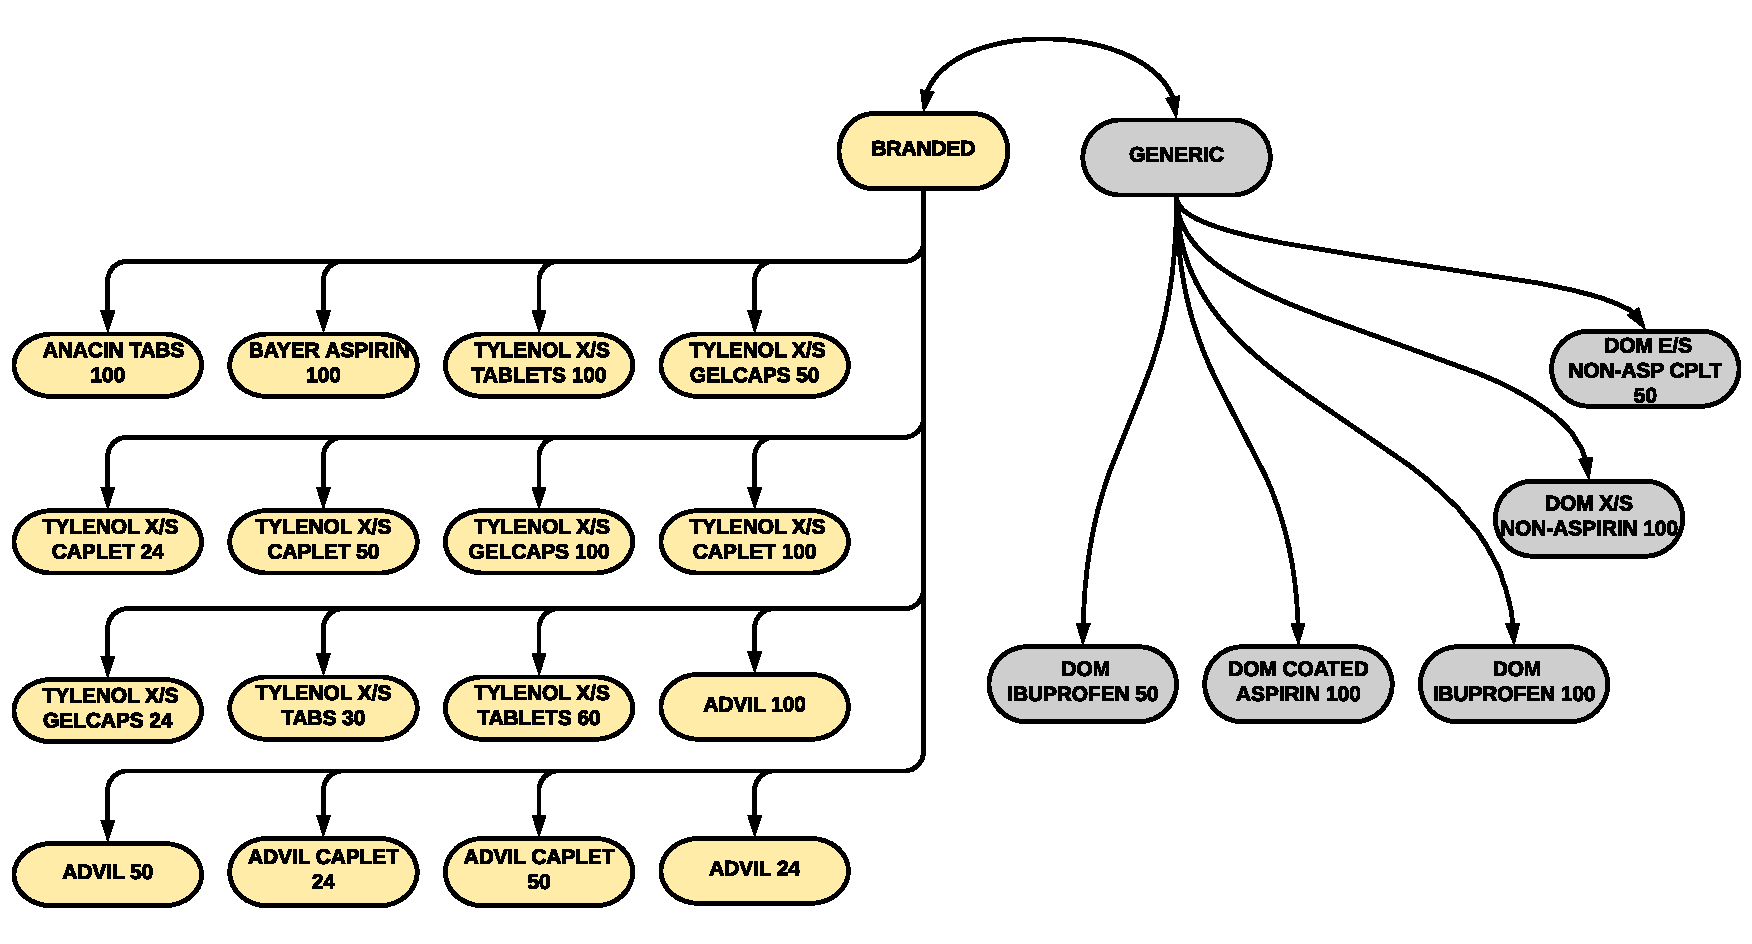
\includegraphics[clip, angle=0, width=1\textwidth]{FIG3.pdf}
	\caption{Tree structure of the brand type nested logit model}\label{app_brand_tree}
\end{figure}

\begin{figure}[H]
	\centering
	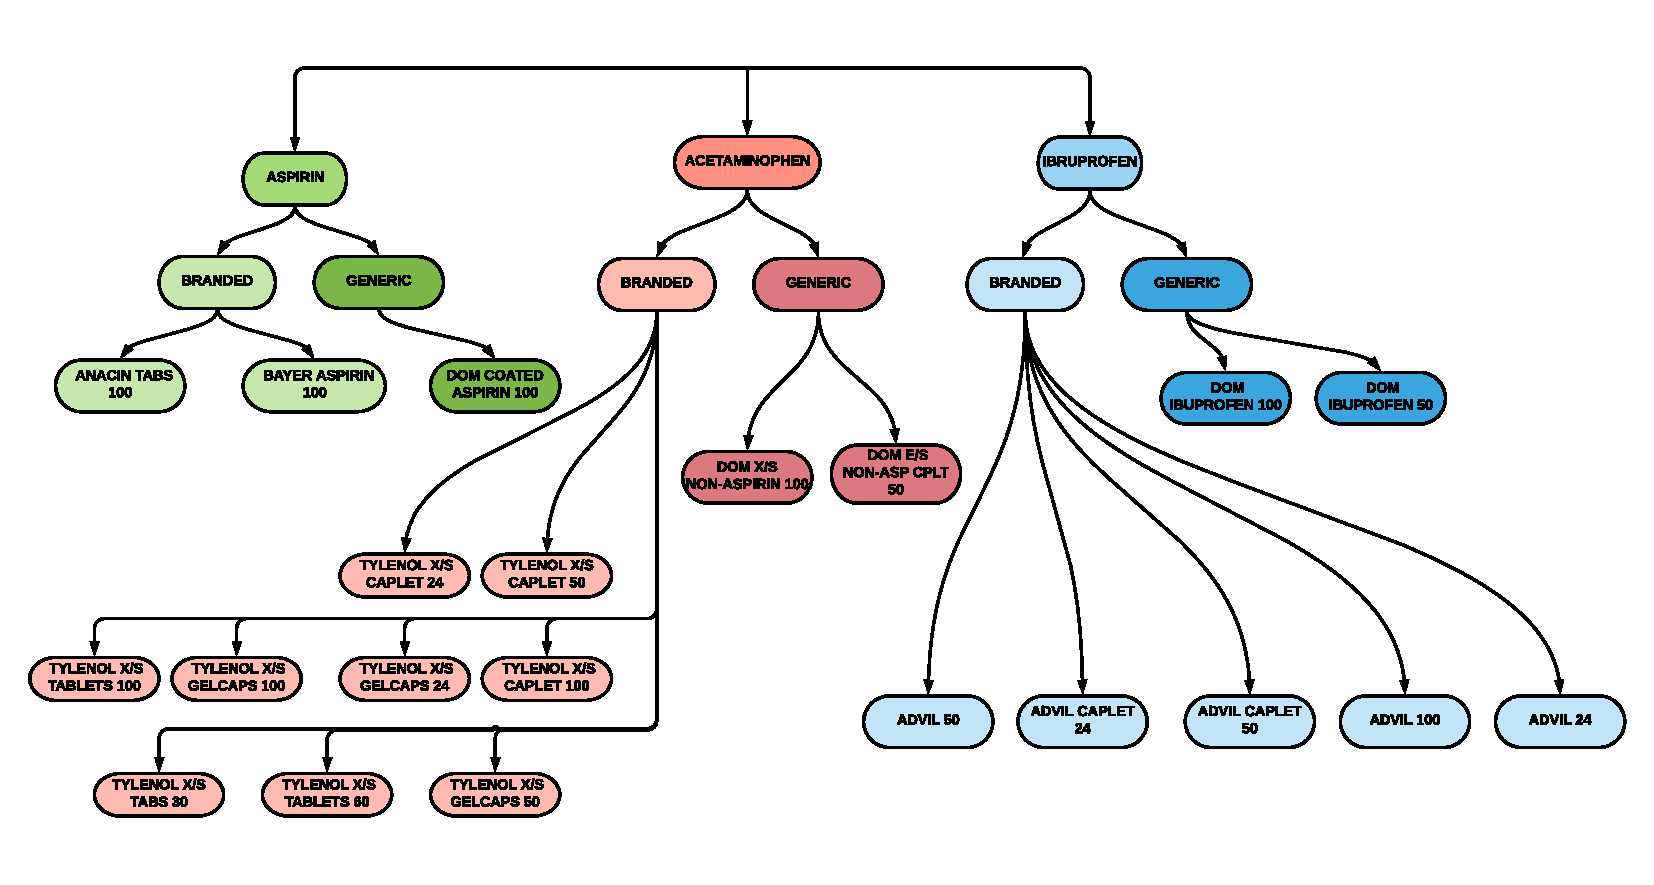
\includegraphics[clip, angle=0, width=1\textwidth]{FIG2.pdf}
	\caption{Tree structure of the double nested logit model}\label{app_double_tree}
\end{figure}

\section{Multinomial Logit Elasticities}  \label{app1}

\begin{figure}[H]
	\centering
	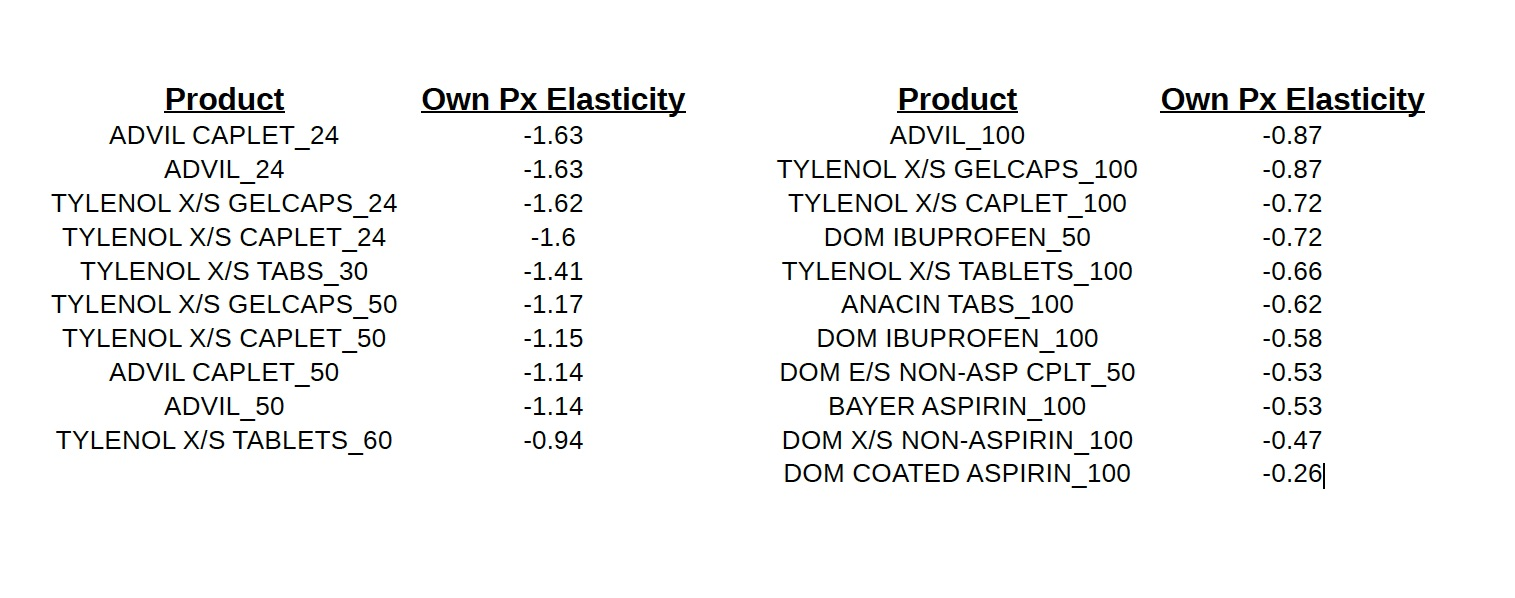
\includegraphics[clip, angle=0, width=1\textwidth]{own_p_elas}
	\caption{Multinomial Logit Elasticities }\label{elas0}
\end{figure}

\section{Nested Logit Elasticities} \label{app2}

\begin{figure}[H]
	\centering
	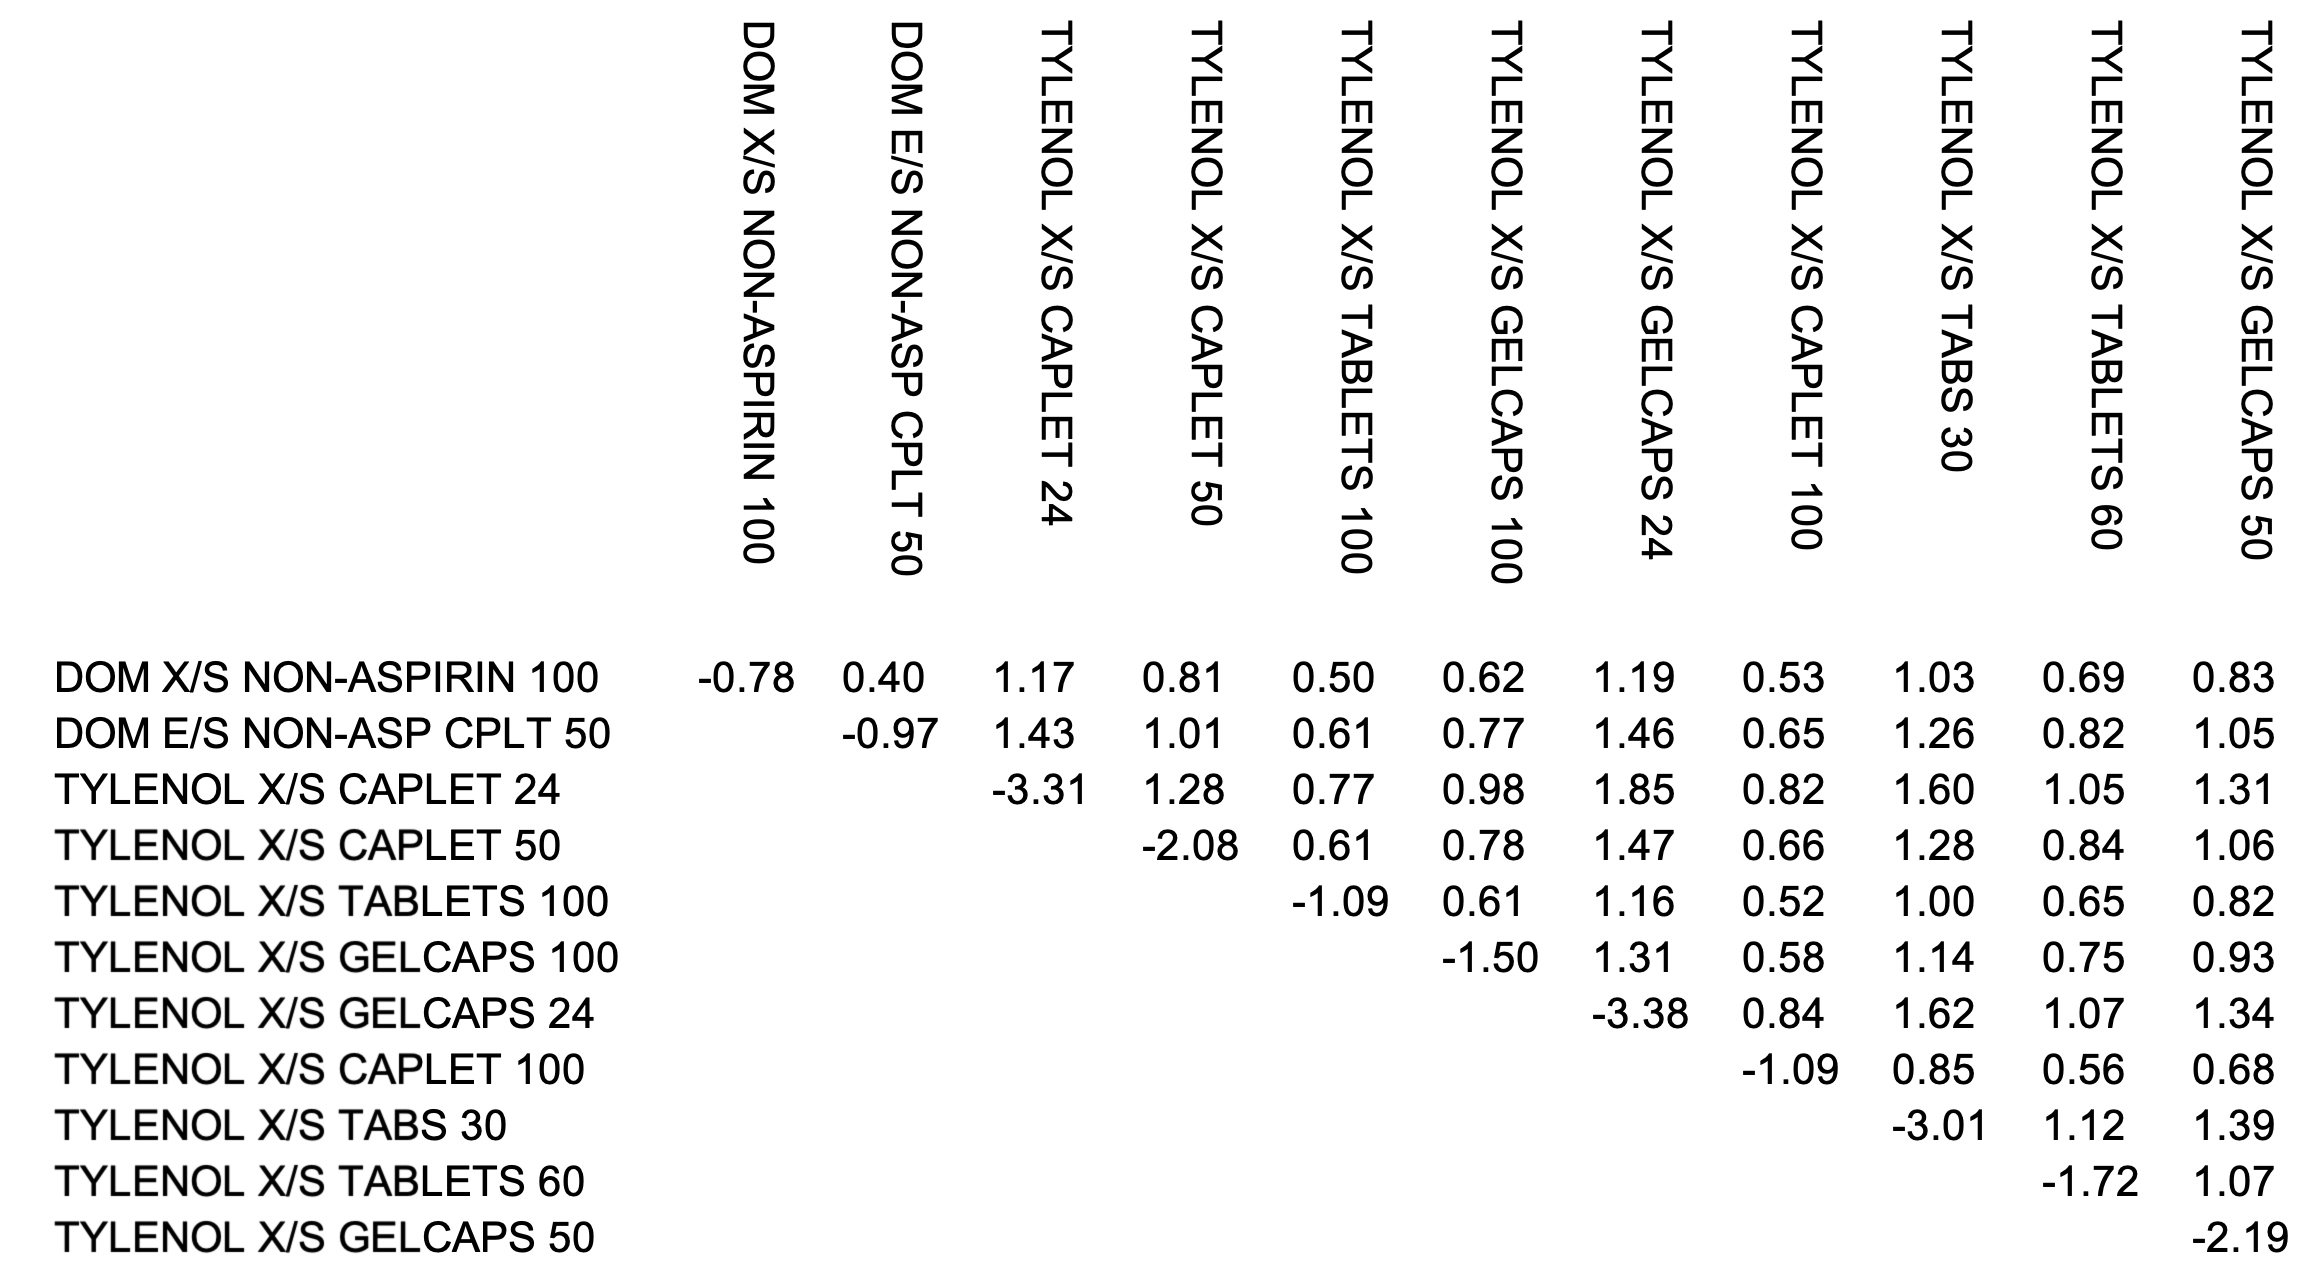
\includegraphics[clip, angle=0, width=1\textwidth]{elas1}
	\caption{Acetaminophen Elasticities }\label{elas1}
\end{figure}

\begin{figure}[H]
	\centering
	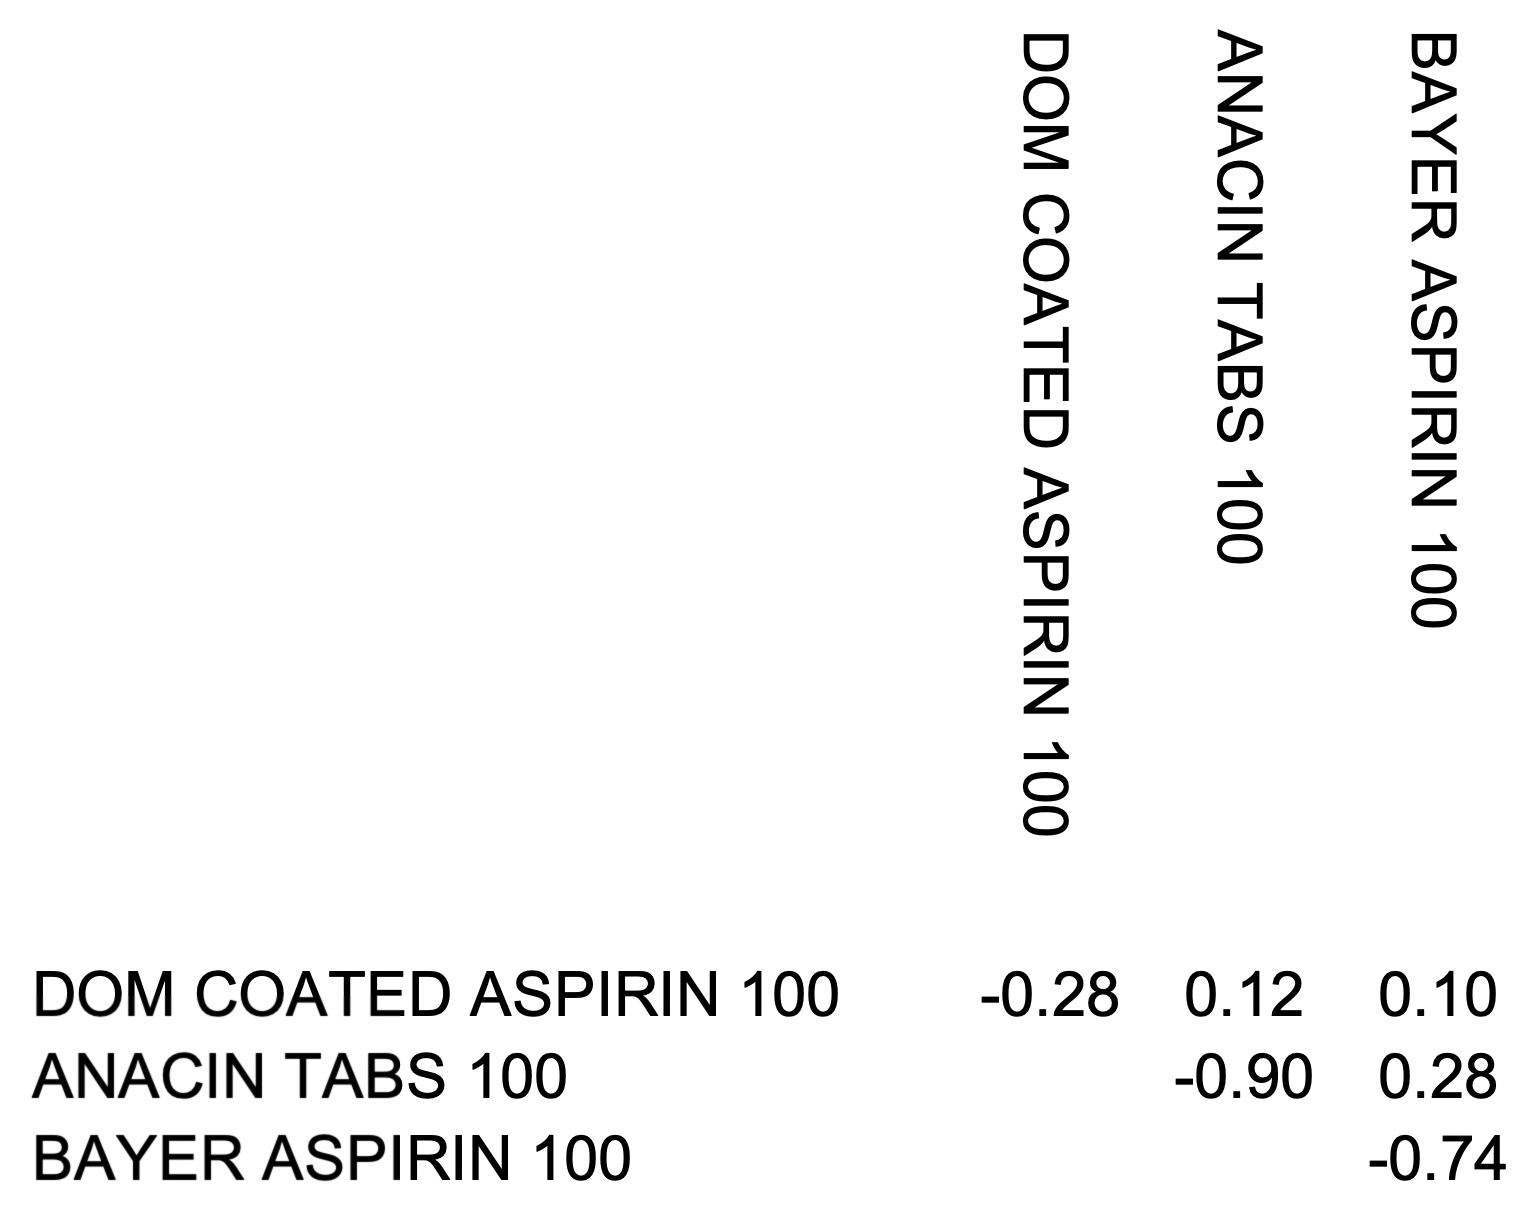
\includegraphics[clip, angle=0, width=7.5cm]{elas2}
	\caption{Aspirin Elasticities }\label{elas2}
\end{figure}

\begin{figure}[H]
	\centering
	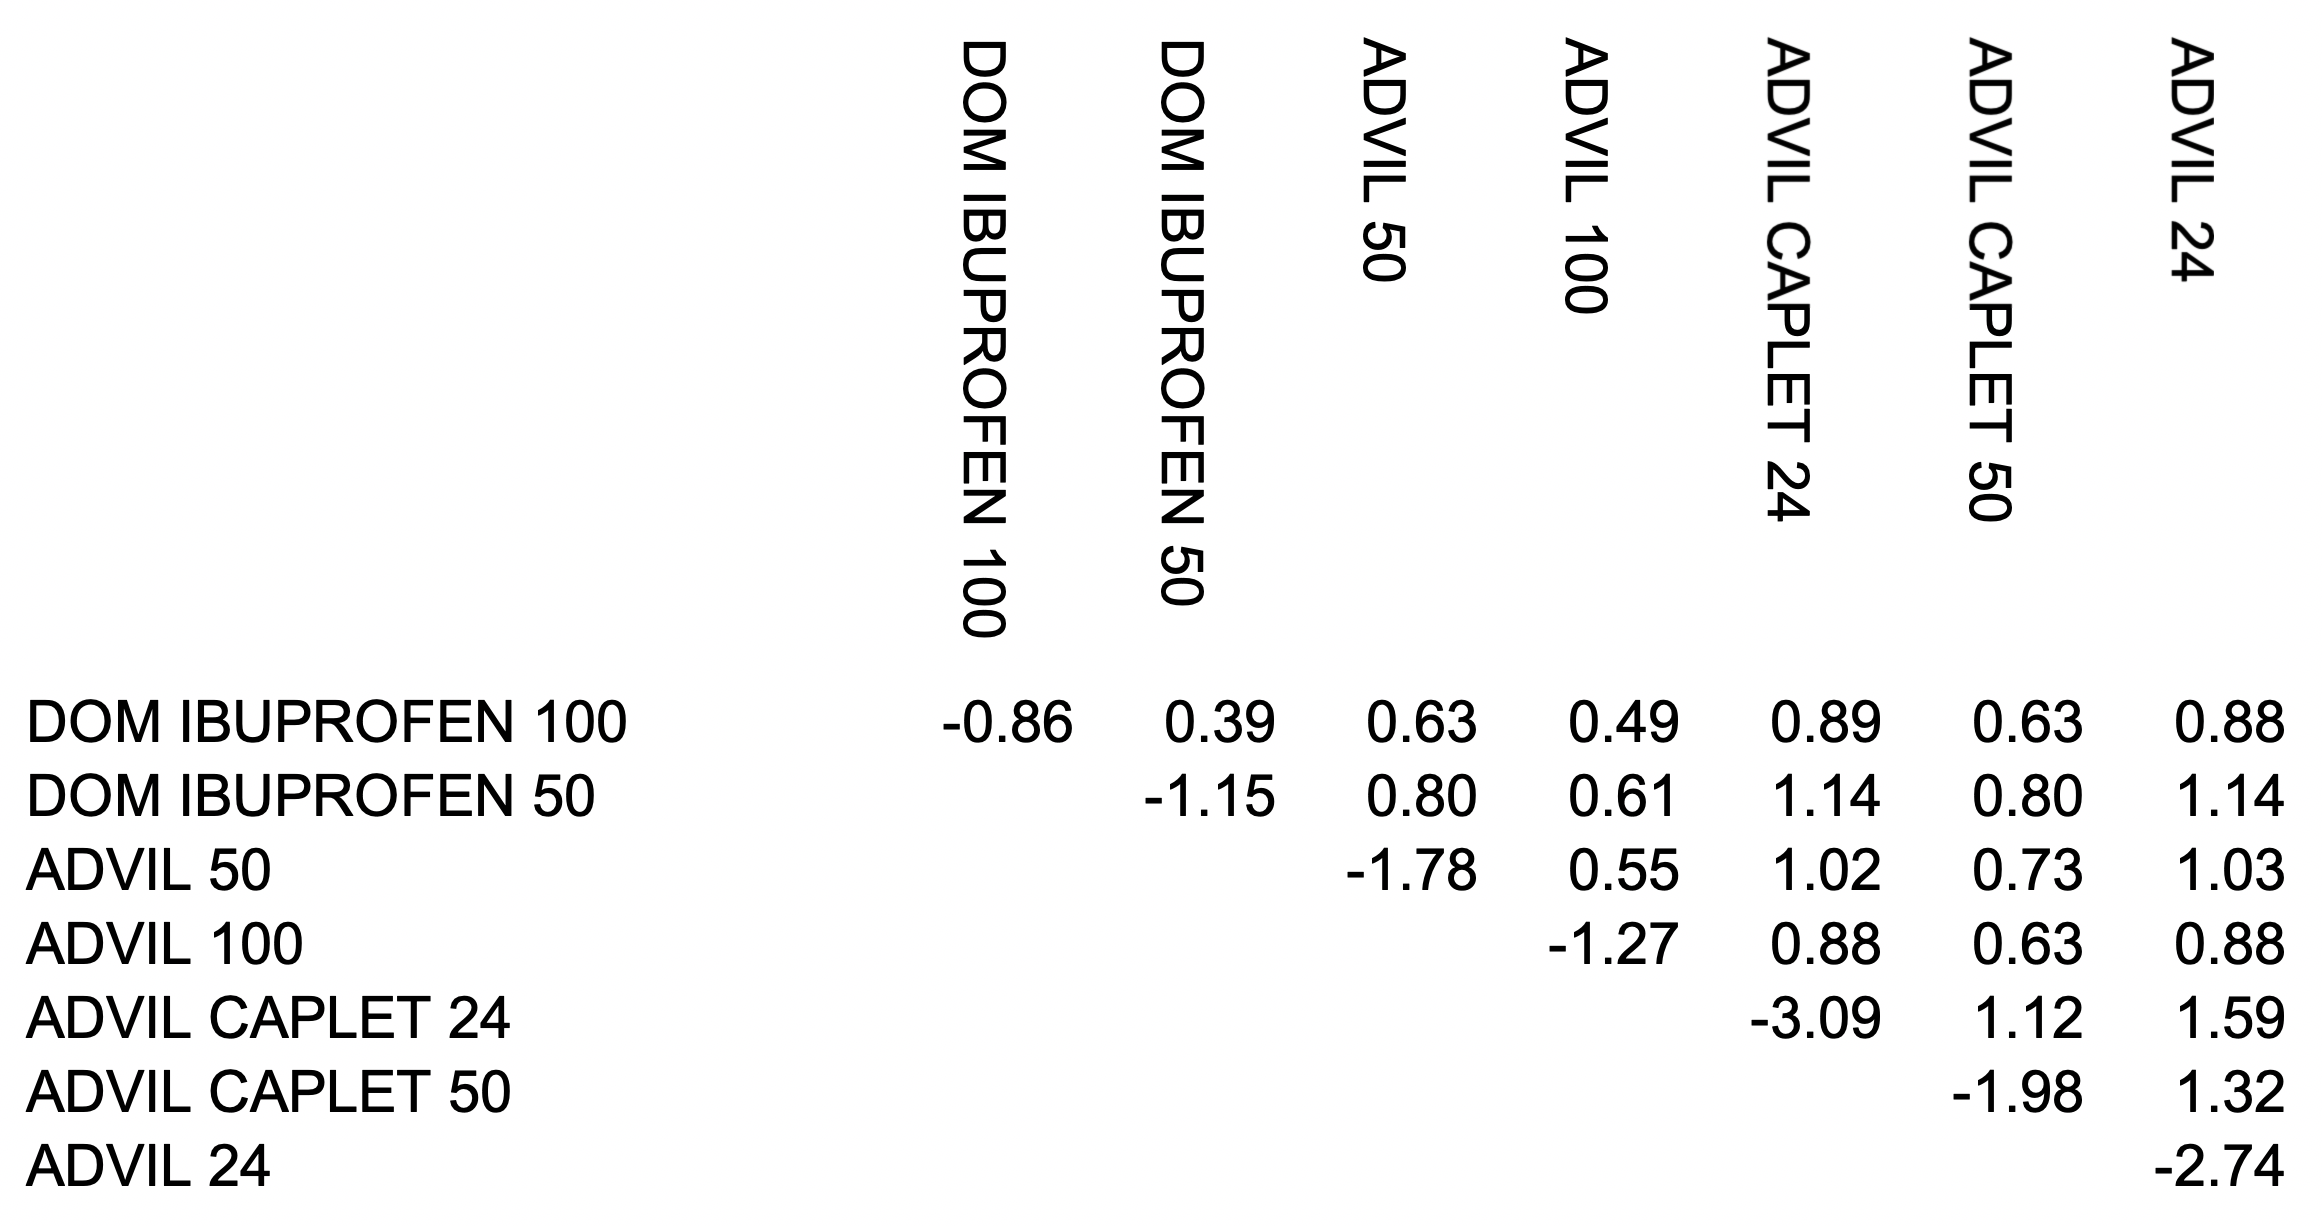
\includegraphics[clip, angle=0, width=12cm]{elas3}
	\caption{Ibuprofen Elasticities }\label{elas3}
\end{figure}

\section{Predicting Wholesale Prices} \label{wholesale_prices}
\begin{table}[H]
	\begin{tabular}{lc} \hline \hline
		\cellcolor{gray!25}  Dependent Variable & \cellcolor{gray!25}  Weekly Wholesale Prices \\ \hline
		Size 1 & -3918852.18 \\
		Size 2 & -3918852.20 \\
		Size 3 & -3918852.21 \\
		Firm 1 & -72029832.25 \\
		Firm 2 & -72029832.21 \\
		Firm 3 & -72029832.23 \\
		Firm 4 & -72029832.22 \\
		Firm 5 & -72029832.23 \\
		Active Ingredient 1 & 24648424.80 \\
		Active Ingredient 2 & 24648424.80 \\
		Active Ingredient 3 & 24648424.80 \\
		USD vs CNY Firm 1 & -0.00*** \\
		USD vs CNY Firm 2 & -0.00*** \\
		USD vs CNY Firm 3 & 0.00*** \\
		USD vs CNY Firm 4 & 0.00*** \\
		USD vs CNY Firm 5 & -0.00*** \\
		USD vs INR Firm 1 & 0.00 \\
		USD vs INR Firm 2 & -0.00*** \\
		USD vs INR Firm 3 & 0.00*** \\
		USD vs INR Firm 4 & 0.00*** \\
		USD vs INR Firm 5 & 0.00*** \\
		EUR vs USD Firm 1 & 0.00*** \\
		EUR vs USD Firm 2 & 0.02*** \\
		EUR vs USD Firm 3 & 0.02*** \\
		EUR vs USD Firm 4 & 0.01*** \\
		EUR vs USD Firm 5 & 0.01*** \\ \hline
		N & 344796.00 \\
		$R^{2}$ & 0.97 \\  \hline \hline
		\multicolumn{2}{c}{Notes: $* p<0.1, ** p<0.05, ***p<0.01$}    
	\end{tabular}
\end{table}

\begin{figure}[H]
	\centering
	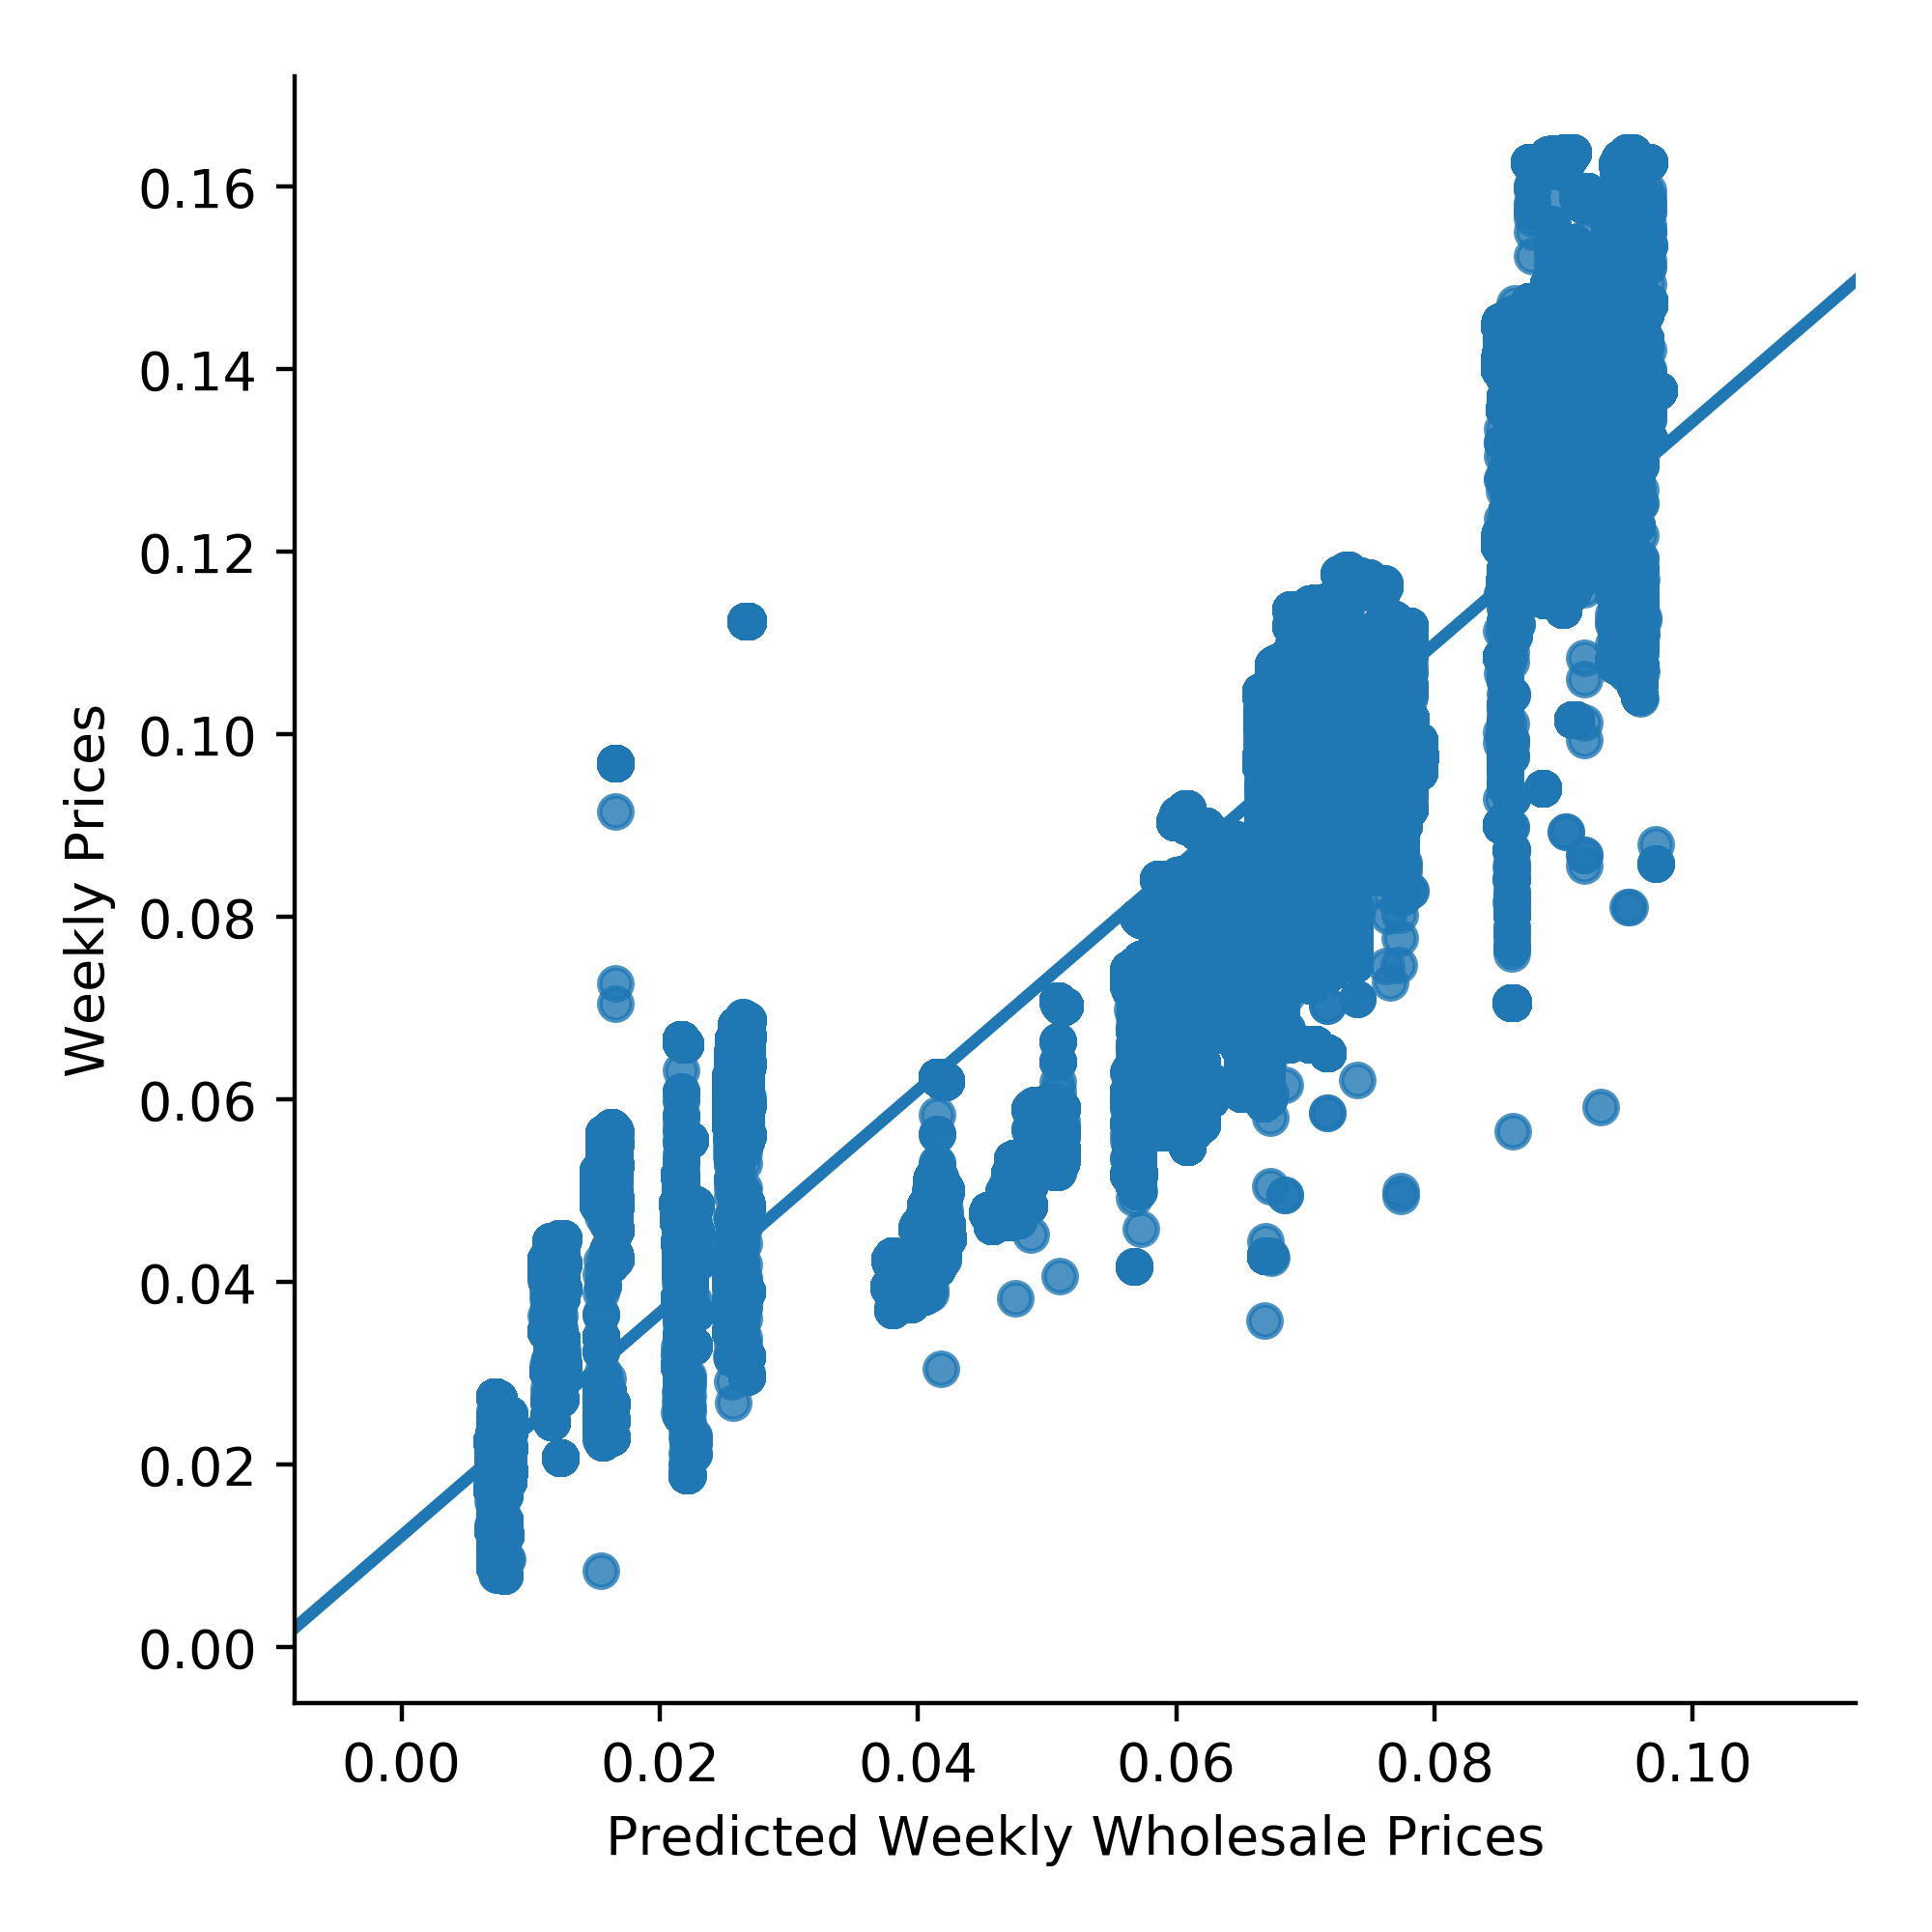
\includegraphics[clip, angle=0, width=12cm]{wholesale_prices}
	\caption{Predicted Weekly Wholesale Prices vs Actual Weekly Retail Prices}\label{wholesale_prices_plot}
\end{figure}

\end{document}
